\documentclass{article}\usepackage[]{graphicx}\usepackage[]{color}
% maxwidth is the original width if it is less than linewidth
% otherwise use linewidth (to make sure the graphics do not exceed the margin)
\makeatletter
\def\maxwidth{ %
  \ifdim\Gin@nat@width>\linewidth
    \linewidth
  \else
    \Gin@nat@width
  \fi
}
\makeatother

\definecolor{fgcolor}{rgb}{0.345, 0.345, 0.345}
\newcommand{\hlnum}[1]{\textcolor[rgb]{0.686,0.059,0.569}{#1}}%
\newcommand{\hlstr}[1]{\textcolor[rgb]{0.192,0.494,0.8}{#1}}%
\newcommand{\hlcom}[1]{\textcolor[rgb]{0.678,0.584,0.686}{\textit{#1}}}%
\newcommand{\hlopt}[1]{\textcolor[rgb]{0,0,0}{#1}}%
\newcommand{\hlstd}[1]{\textcolor[rgb]{0.345,0.345,0.345}{#1}}%
\newcommand{\hlkwa}[1]{\textcolor[rgb]{0.161,0.373,0.58}{\textbf{#1}}}%
\newcommand{\hlkwb}[1]{\textcolor[rgb]{0.69,0.353,0.396}{#1}}%
\newcommand{\hlkwc}[1]{\textcolor[rgb]{0.333,0.667,0.333}{#1}}%
\newcommand{\hlkwd}[1]{\textcolor[rgb]{0.737,0.353,0.396}{\textbf{#1}}}%
\let\hlipl\hlkwb

\usepackage{framed}
\makeatletter
\newenvironment{kframe}{%
 \def\at@end@of@kframe{}%
 \ifinner\ifhmode%
  \def\at@end@of@kframe{\end{minipage}}%
  \begin{minipage}{\columnwidth}%
 \fi\fi%
 \def\FrameCommand##1{\hskip\@totalleftmargin \hskip-\fboxsep
 \colorbox{shadecolor}{##1}\hskip-\fboxsep
     % There is no \\@totalrightmargin, so:
     \hskip-\linewidth \hskip-\@totalleftmargin \hskip\columnwidth}%
 \MakeFramed {\advance\hsize-\width
   \@totalleftmargin\z@ \linewidth\hsize
   \@setminipage}}%
 {\par\unskip\endMakeFramed%
 \at@end@of@kframe}
\makeatother

\definecolor{shadecolor}{rgb}{.97, .97, .97}
\definecolor{messagecolor}{rgb}{0, 0, 0}
\definecolor{warningcolor}{rgb}{1, 0, 1}
\definecolor{errorcolor}{rgb}{1, 0, 0}
\newenvironment{knitrout}{}{} % an empty environment to be redefined in TeX

\usepackage{alltt}
\usepackage[sc]{mathpazo}
\renewcommand{\sfdefault}{lmss}
\renewcommand{\ttdefault}{lmtt}
\usepackage[T1]{fontenc}
\usepackage{geometry}
\geometry{verbose,tmargin=2.5cm,bmargin=2.5cm,lmargin=2.5cm,rmargin=2.5cm}
\setcounter{secnumdepth}{2}
\setcounter{tocdepth}{2}
\usepackage[unicode=true,pdfusetitle,
 bookmarks=true,bookmarksnumbered=true,bookmarksopen=true,bookmarksopenlevel=2,
 breaklinks=false,pdfborder={0 0 1},backref=false,colorlinks=false]
 {hyperref}
\hypersetup{
 pdfstartview={XYZ null null 1}}

\makeatletter
%%%%%%%%%%%%%%%%%%%%%%%%%%%%%% User specified LaTeX commands.
\renewcommand{\textfraction}{0.05}
\renewcommand{\topfraction}{0.8}
\renewcommand{\bottomfraction}{0.8}
\renewcommand{\floatpagefraction}{0.75}

\makeatother
\IfFileExists{upquote.sty}{\usepackage{upquote}}{}
\begin{document}



\title{}



\maketitle
The results below are generated from an R script.

\begin{knitrout}
\definecolor{shadecolor}{rgb}{0.969, 0.969, 0.969}\color{fgcolor}\begin{kframe}
\begin{alltt}
\hlcom{# Analysis}
\hlcom{# Scott Cohn + Ruja Kambli}

\hlcom{# Libraries ---------------------------------------------------------------}

\hlkwd{library}\hlstd{(dplyr)}
\hlkwd{library}\hlstd{(tidyverse)} \hlcom{# duh.}
\hlkwd{library}\hlstd{(ggplot2)} \hlcom{# plotting}
\hlkwd{library}\hlstd{(gridExtra)} \hlcom{# plotting options}
\hlkwd{library}\hlstd{(ggsci)}  \hlcom{# plot color palette}
\hlkwd{library}\hlstd{(ggthemes)} \hlcom{# Themes}
\hlkwd{library}\hlstd{(bbplot)} \hlcom{# plot style}
\hlkwd{library}\hlstd{(readr)} \hlcom{# import csv}
\hlkwd{library}\hlstd{(lmtest)} \hlcom{# BP test}
\hlkwd{library}\hlstd{(scales)} \hlcom{# Scale x-axis}
\hlkwd{library}\hlstd{(MASS)}
\hlkwd{library}\hlstd{(faraway)} \hlcom{# Box-Cox transform / vif}

\hlcom{# Colors}
\hlstd{COLA} \hlkwb{<-} \hlkwd{c}\hlstd{(}\hlstr{"#99d8c9"}\hlstd{,}\hlstr{"#66c2a4"}\hlstd{,}\hlstr{"#41ae76"}\hlstd{,} \hlstr{"#238b45"}\hlstd{,} \hlstr{"#005824"}\hlstd{)}
\hlstd{COLB} \hlkwb{<-} \hlkwd{c}\hlstd{(}\hlstr{"#4eb3d3"}\hlstd{,} \hlstr{"#2b8cbe"}\hlstd{,} \hlstr{"#0868ac"}\hlstd{,}\hlstr{"#084081"}\hlstd{)}

\hlcom{# Import Data -------------------------------------------------------------}
\hlstd{life_exp_full} \hlkwb{<-} \hlkwd{read_csv}\hlstd{(}\hlstr{"data/life_exp_full.csv"}\hlstd{)}
\end{alltt}


{\ttfamily\noindent\itshape\color{messagecolor}{\#\# Parsed with column specification:\\\#\# cols(\\\#\#\ \  Country = col\_character(),\\\#\#\ \  `Birth Rate` = col\_double(),\\\#\#\ \  `Cancer Rate` = col\_double(),\\\#\#\ \  `Dengue Cases` = col\_double(),\\\#\#\ \  EPI = col\_double(),\\\#\#\ \  GDP = col\_double(),\\\#\#\ \  `Health Expenditure` = col\_double(),\\\#\#\ \  `Heart Disease Rate` = col\_double(),\\\#\#\ \  Population = col\_double(),\\\#\#\ \  Area = col\_double(),\\\#\#\ \  `Pop Density` = col\_double(),\\\#\#\ \  `Stroke Rate` = col\_double(),\\\#\#\ \  `Life Expectancy` = col\_double()\\\#\# )}}\begin{alltt}
\hlcom{# Data Transformations ----------------------------------------------------}

\hlcom{# Capitalize letters in Country var}
\hlcom{# Not perfect, but good enough}
\hlstd{simpleCap} \hlkwb{<-} \hlkwa{function}\hlstd{(}\hlkwc{x}\hlstd{) \{}
  \hlstd{s} \hlkwb{<-} \hlkwd{strsplit}\hlstd{(x,} \hlstr{" "}\hlstd{)[[}\hlnum{1}\hlstd{]]}
  \hlkwd{paste}\hlstd{(}\hlkwd{toupper}\hlstd{(}\hlkwd{substring}\hlstd{(s,} \hlnum{1}\hlstd{,}\hlnum{1}\hlstd{)),} \hlkwd{substring}\hlstd{(s,} \hlnum{2}\hlstd{),}
        \hlkwc{sep} \hlstd{=} \hlstr{""}\hlstd{,} \hlkwc{collapse} \hlstd{=} \hlstr{" "}\hlstd{)}
\hlstd{\}}

\hlstd{life_exp_full} \hlkwb{<-} \hlstd{life_exp_full} \hlopt
  \hlkwd{mutate}\hlstd{(}\hlkwc{Country} \hlstd{=} \hlkwd{apply}\hlstd{(life_exp_full,} \hlnum{1}\hlstd{, simpleCap))}

\hlcom{# Visualizations ----------------------------------------------------------}

\hlcom{# Top 10 life exp by country}
\hlstd{topten_lifeexp_country} \hlkwb{<-} \hlstd{life_exp_full} \hlopt
  \hlkwd{arrange}\hlstd{(}\hlkwd{desc}\hlstd{(`Life Expectancy`))} \hlopt
  \hlkwd{slice}\hlstd{(}\hlnum{1}\hlopt{:}\hlnum{10}\hlstd{)} \hlopt
  \hlkwd{ggplot}\hlstd{(}\hlkwd{aes}\hlstd{(}\hlkwc{x} \hlstd{=} \hlkwd{reorder}\hlstd{(Country, `Life Expectancy`),}
             \hlkwc{y} \hlstd{= `Life Expectancy`))} \hlopt{+}
  \hlkwd{geom_bar}\hlstd{(}\hlkwc{stat} \hlstd{=} \hlstr{'identity'}\hlstd{,}
           \hlkwc{fill} \hlstd{=} \hlstr{"#1380A1"}\hlstd{)} \hlopt{+}
  \hlcom{#scale_fill_d3() +}
  \hlkwd{coord_flip}\hlstd{()} \hlopt{+}
  \hlkwd{scale_y_continuous}\hlstd{(}
    \hlkwc{limits} \hlstd{=} \hlkwd{c}\hlstd{(}\hlnum{0}\hlstd{,} \hlnum{85}\hlstd{),}
    \hlkwc{breaks} \hlstd{=} \hlkwd{seq}\hlstd{(}\hlnum{0}\hlstd{,} \hlnum{80}\hlstd{,} \hlkwc{by} \hlstd{=} \hlnum{20}\hlstd{),}
    \hlkwc{labels} \hlstd{=} \hlkwd{c}\hlstd{(}\hlstr{"0"}\hlstd{,} \hlstr{"20"}\hlstd{,} \hlstr{"40"}\hlstd{,} \hlstr{"60"}\hlstd{,} \hlstr{"80 years"}\hlstd{)}
  \hlstd{)} \hlopt{+}
  \hlkwd{geom_hline}\hlstd{(}\hlkwc{yintercept} \hlstd{=} \hlnum{0}\hlstd{,}
             \hlkwc{size} \hlstd{=} \hlnum{1}\hlstd{,}
             \hlkwc{color} \hlstd{=} \hlstr{"#333333"}\hlstd{)} \hlopt{+}
  \hlkwd{geom_label}\hlstd{(}
    \hlkwd{aes}\hlstd{(}\hlkwc{label} \hlstd{=} \hlkwd{round}\hlstd{(`Life Expectancy`,} \hlnum{0}\hlstd{)),}
    \hlkwc{hjust} \hlstd{=} \hlnum{1}\hlstd{,}
    \hlkwc{vjust} \hlstd{=} \hlnum{0.5}\hlstd{,}
    \hlkwc{colour} \hlstd{=} \hlstr{"white"}\hlstd{,}
    \hlkwc{fill} \hlstd{=} \hlnum{NA}\hlstd{,}
    \hlkwc{label.size} \hlstd{=} \hlnum{NA}\hlstd{,}
    \hlkwc{family} \hlstd{=} \hlstr{"Helvetica"}\hlstd{,}
    \hlkwc{size} \hlstd{=} \hlnum{6}
  \hlstd{)} \hlopt{+}
  \hlkwd{bbc_style}\hlstd{()} \hlopt{+}
  \hlkwd{labs}\hlstd{(}\hlkwc{title} \hlstd{=} \hlstr{"Life Expectancy"}\hlstd{,}
       \hlkwc{subtitle} \hlstd{=} \hlstr{"Top 10 Countries"}\hlstd{)}

\hlcom{# Save graph}
\hlkwd{finalise_plot}\hlstd{(}\hlkwc{plot_name} \hlstd{= topten_lifeexp_country,}
              \hlkwc{source} \hlstd{=} \hlstr{"Source: JNYH/Project Luther"}\hlstd{,}
              \hlkwc{save_filepath} \hlstd{=} \hlstr{"figures/topten_lifeexp_country.pdf"}\hlstd{,}
              \hlkwc{width_pixels} \hlstd{=} \hlnum{640}\hlstd{,}
              \hlkwc{height_pixels} \hlstd{=} \hlnum{450}\hlstd{)}
\end{alltt}
\end{kframe}

{\centering 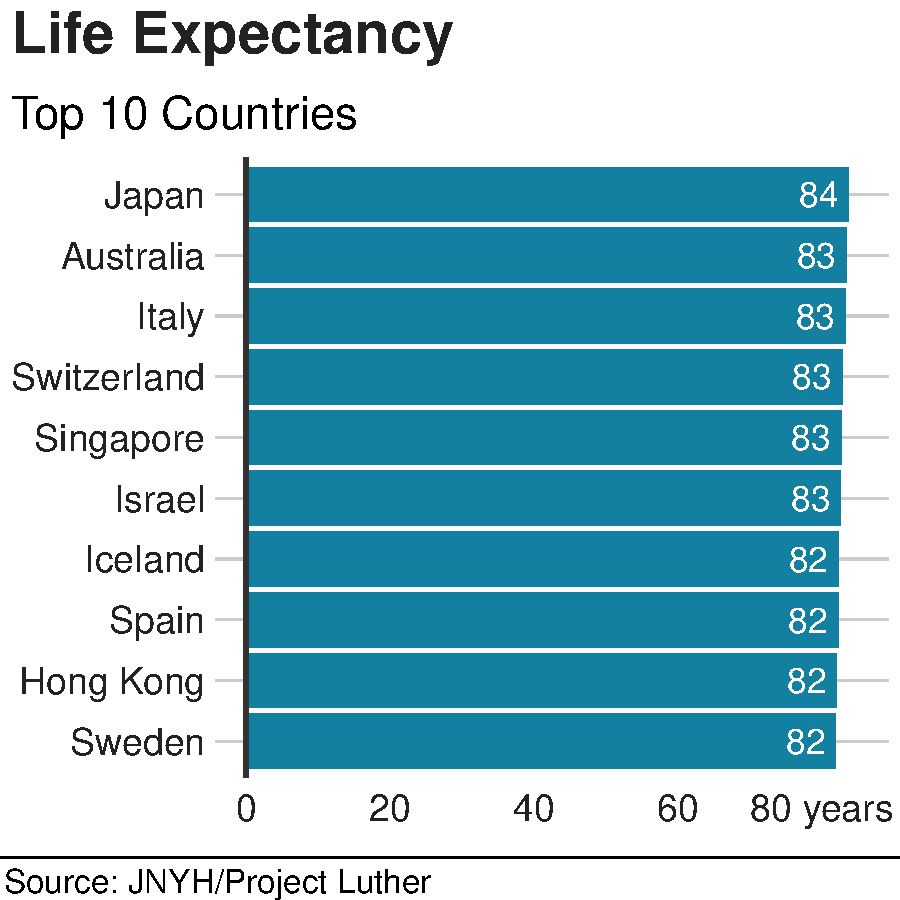
\includegraphics[width=.6\linewidth]{figure/Analysis-Rnwauto-report-1} 

}


\begin{kframe}\begin{alltt}
              \hlcom{#logo_image_path = "placeholder.png")}

\hlcom{# Bottom 10 life exp by country}
\hlcom{# life_exp_full %>% drop_na(`Life Expectancy`) %>% nrow() = 201 rows w/out NA}
\hlstd{bottomten_lifeexp_country} \hlkwb{<-} \hlstd{life_exp_full} \hlopt
  \hlkwd{drop_na}\hlstd{(`Life Expectancy`)} \hlopt
  \hlkwd{arrange}\hlstd{(}\hlkwd{desc}\hlstd{(`Life Expectancy`))} \hlopt
  \hlkwd{slice}\hlstd{(}\hlnum{192}\hlopt{:}\hlnum{201}\hlstd{)} \hlopt
  \hlkwd{ggplot}\hlstd{(}\hlkwd{aes}\hlstd{(}\hlkwc{x} \hlstd{=} \hlkwd{reorder}\hlstd{(Country,} \hlopt{-}\hlstd{`Life Expectancy`),}
             \hlkwc{y} \hlstd{= `Life Expectancy`))} \hlopt{+}
  \hlkwd{geom_bar}\hlstd{(}\hlkwc{stat} \hlstd{=} \hlstr{'identity'}\hlstd{,}
           \hlkwc{fill} \hlstd{=} \hlstr{"#1380A1"}\hlstd{)} \hlopt{+}
  \hlcom{#scale_fill_d3() +}
  \hlkwd{coord_flip}\hlstd{()} \hlopt{+}
  \hlkwd{scale_y_continuous}\hlstd{(}
    \hlkwc{limits} \hlstd{=} \hlkwd{c}\hlstd{(}\hlnum{0}\hlstd{,} \hlnum{85}\hlstd{),}
    \hlkwc{breaks} \hlstd{=} \hlkwd{seq}\hlstd{(}\hlnum{0}\hlstd{,} \hlnum{80}\hlstd{,} \hlkwc{by} \hlstd{=} \hlnum{20}\hlstd{),}
    \hlkwc{labels} \hlstd{=} \hlkwd{c}\hlstd{(}\hlstr{"0"}\hlstd{,} \hlstr{"20"}\hlstd{,} \hlstr{"40"}\hlstd{,} \hlstr{"60"}\hlstd{,} \hlstr{"80 years"}\hlstd{)}
  \hlstd{)} \hlopt{+}
  \hlkwd{geom_hline}\hlstd{(}\hlkwc{yintercept} \hlstd{=} \hlnum{0}\hlstd{,}
             \hlkwc{size} \hlstd{=} \hlnum{1}\hlstd{,}
             \hlkwc{color} \hlstd{=} \hlstr{"#333333"}\hlstd{)} \hlopt{+}
  \hlkwd{geom_label}\hlstd{(}
    \hlkwd{aes}\hlstd{(}\hlkwc{label} \hlstd{=} \hlkwd{round}\hlstd{(`Life Expectancy`,} \hlnum{0}\hlstd{)),}
    \hlkwc{hjust} \hlstd{=} \hlnum{1}\hlstd{,}
    \hlkwc{vjust} \hlstd{=} \hlnum{0.5}\hlstd{,}
    \hlkwc{colour} \hlstd{=} \hlstr{"white"}\hlstd{,}
    \hlkwc{fill} \hlstd{=} \hlnum{NA}\hlstd{,}
    \hlkwc{label.size} \hlstd{=} \hlnum{NA}\hlstd{,}
    \hlkwc{family} \hlstd{=} \hlstr{"Helvetica"}\hlstd{,}
    \hlkwc{size} \hlstd{=} \hlnum{6}
  \hlstd{)} \hlopt{+}
  \hlkwd{bbc_style}\hlstd{()} \hlopt{+}
  \hlkwd{labs}\hlstd{(}\hlkwc{title} \hlstd{=} \hlstr{"Life Expectancy"}\hlstd{,}
       \hlkwc{subtitle} \hlstd{=} \hlstr{"Bottom 10 Countries"}\hlstd{)}

\hlcom{# Save graph}
\hlkwd{finalise_plot}\hlstd{(}\hlkwc{plot_name} \hlstd{= bottomten_lifeexp_country,}
              \hlkwc{source} \hlstd{=} \hlstr{"Source: JNYH/Project Luther"}\hlstd{,}
              \hlkwc{save_filepath} \hlstd{=} \hlstr{"figures/bottomten_lifeexp_country.pdf"}\hlstd{,}
              \hlkwc{width_pixels} \hlstd{=} \hlnum{640}\hlstd{,}
              \hlkwc{height_pixels} \hlstd{=} \hlnum{450}\hlstd{)}
\end{alltt}
\end{kframe}

{\centering 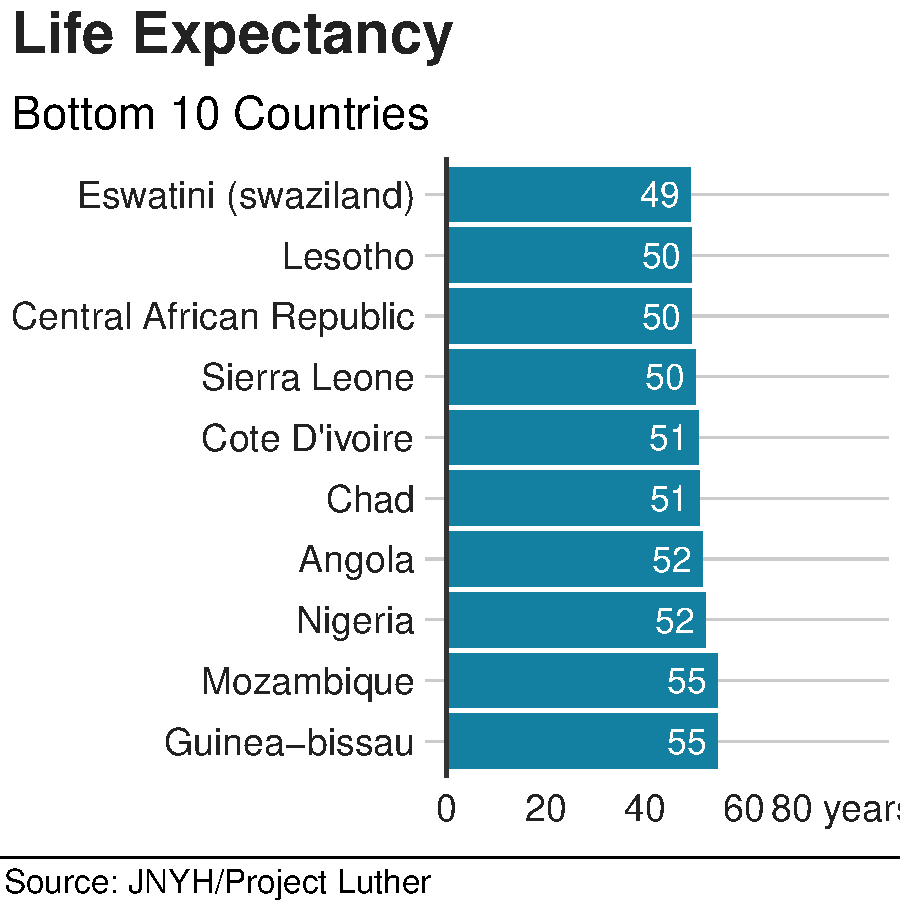
\includegraphics[width=.6\linewidth]{figure/Analysis-Rnwauto-report-2} 

}


\begin{kframe}\begin{alltt}
\hlcom{#logo_image_path = "placeholder.png")}

\hlcom{# Distribution of Life Expectancy, Histogram}
\hlstd{lifeexp_distro} \hlkwb{<-} \hlstd{life_exp_full} \hlopt
  \hlkwd{ggplot}\hlstd{(}\hlkwd{aes}\hlstd{(}\hlkwc{x} \hlstd{= `Life Expectancy`))} \hlopt{+}
  \hlkwd{geom_histogram}\hlstd{(}\hlkwc{binwidth} \hlstd{=} \hlnum{5}\hlstd{,}
                 \hlkwc{color} \hlstd{=} \hlstr{"white"}\hlstd{,}
                 \hlkwc{fill} \hlstd{=} \hlstr{"#1380A1"}\hlstd{)} \hlopt{+}
  \hlkwd{geom_hline}\hlstd{(}\hlkwc{yintercept} \hlstd{=} \hlnum{0}\hlstd{,}
             \hlkwc{size} \hlstd{=} \hlnum{1}\hlstd{,}
             \hlkwc{color} \hlstd{=} \hlstr{"#333333"}\hlstd{)} \hlopt{+}
  \hlkwd{bbc_style}\hlstd{()} \hlopt{+}
  \hlkwd{scale_x_continuous}\hlstd{(}
    \hlkwc{limits} \hlstd{=} \hlkwd{c}\hlstd{(}\hlnum{40}\hlstd{,} \hlnum{95}\hlstd{),}
    \hlkwc{breaks} \hlstd{=} \hlkwd{seq}\hlstd{(}\hlnum{40}\hlstd{,} \hlnum{90}\hlstd{,} \hlkwc{by} \hlstd{=} \hlnum{10}\hlstd{),}
    \hlkwc{labels} \hlstd{=} \hlkwd{c}\hlstd{(}\hlstr{"40"}\hlstd{,} \hlstr{"50"}\hlstd{,} \hlstr{"60"}\hlstd{,} \hlstr{"70"}\hlstd{,} \hlstr{"80"}\hlstd{,} \hlstr{"90 years"}\hlstd{)}
  \hlstd{)} \hlopt{+}
  \hlkwd{labs}\hlstd{(}\hlkwc{title} \hlstd{=} \hlstr{"How life expectancy varies"}\hlstd{,}
       \hlkwc{subtitle} \hlstd{=} \hlstr{"Distribution of life expectancy"}\hlstd{)}

\hlcom{# Save graph}
\hlkwd{finalise_plot}\hlstd{(}\hlkwc{plot_name} \hlstd{= lifeexp_distro,}
              \hlkwc{source} \hlstd{=} \hlstr{"Source: JNYH/Project Luther"}\hlstd{,}
              \hlkwc{save_filepath} \hlstd{=} \hlstr{"figures/lifeexp_distro.pdf"}\hlstd{,}
              \hlkwc{width_pixels} \hlstd{=} \hlnum{640}\hlstd{,}
              \hlkwc{height_pixels} \hlstd{=} \hlnum{450}\hlstd{)}
\end{alltt}


{\ttfamily\noindent\color{warningcolor}{\#\# Warning: Removed 47 rows containing non-finite values (stat\_bin).}}

{\ttfamily\noindent\color{warningcolor}{\#\# Warning: Removed 2 rows containing missing values (geom\_bar).}}\end{kframe}

{\centering 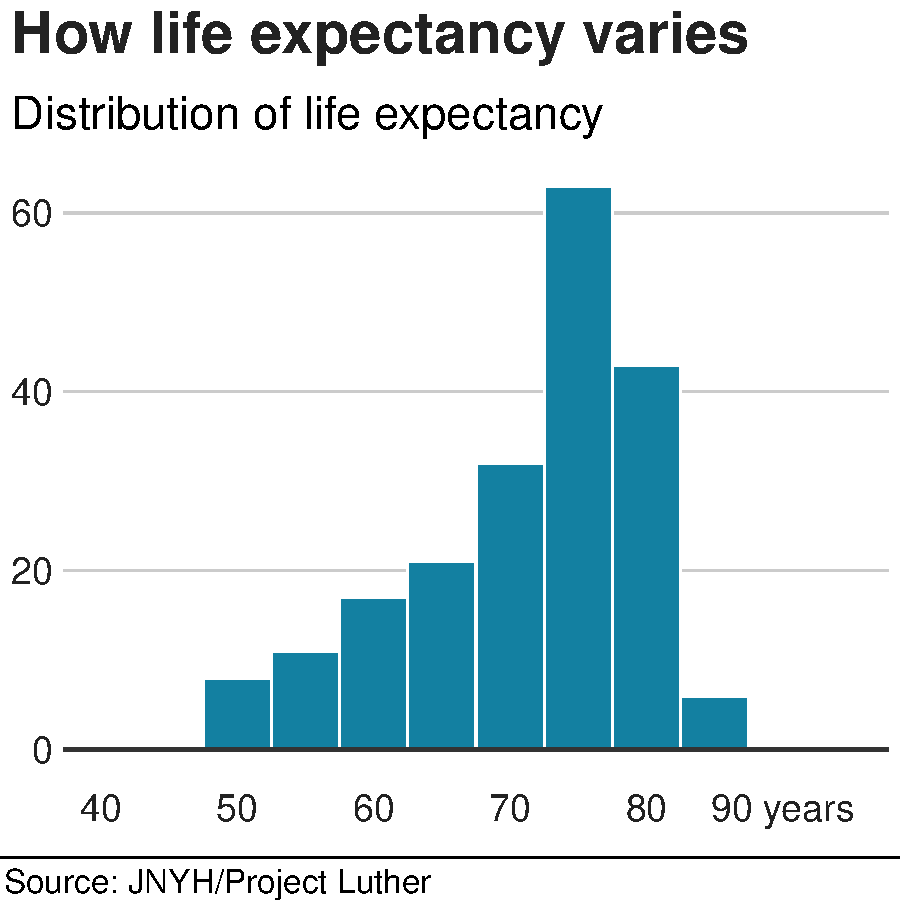
\includegraphics[width=.6\linewidth]{figure/Analysis-Rnwauto-report-3} 

}


\begin{kframe}\begin{alltt}
\hlcom{#logo_image_path = "placeholder.png")}

\hlcom{# Life exp vs Birth Rate}
\hlstd{life_exp_full} \hlopt
  \hlkwd{ggplot}\hlstd{(}\hlkwd{aes}\hlstd{(}\hlkwc{x} \hlstd{= `Birth Rate`,}
             \hlkwc{y} \hlstd{= `Life Expectancy`))} \hlopt{+}
             \hlkwd{xlab}\hlstd{(}\hlstr{"Birth Rate per 1000 People"}\hlstd{)} \hlopt{+}       \hlcom{#RK I tried labelling these axes multiple times, not sure why it isn't showing up? }
             \hlkwd{ylab}\hlstd{(}\hlstr{"Life Expectancy"}\hlstd{)} \hlopt{+}
  \hlkwd{geom_point}\hlstd{(}\hlkwc{color} \hlstd{=} \hlstr{"#1380A1"}\hlstd{)} \hlopt{+}
  \hlkwd{geom_hline}\hlstd{(}\hlkwc{yintercept} \hlstd{=} \hlnum{0}\hlstd{,}
             \hlkwc{size} \hlstd{=} \hlnum{1}\hlstd{,}
             \hlkwc{color} \hlstd{=} \hlstr{"#333333"}\hlstd{)} \hlopt{+}
  \hlcom{#scale_color_d3() +}
  \hlkwd{bbc_style}\hlstd{()} \hlopt{+}
  \hlkwd{labs}\hlstd{(}\hlkwc{title} \hlstd{=} \hlstr{"How long can we expect to live?"}\hlstd{,}
       \hlkwc{subtitle} \hlstd{=} \hlstr{"Birth Rate vs. Life Expectancy"}\hlstd{,}
       \hlkwc{ylab} \hlstd{=} \hlstr{"Life Expectancy"}\hlstd{,}
       \hlkwc{xlab} \hlstd{=} \hlstr{"Births Per 1000 People"}\hlstd{)}
\end{alltt}


{\ttfamily\noindent\color{warningcolor}{\#\# Warning: Removed 54 rows containing missing values (geom\_point).}}\end{kframe}

{\centering 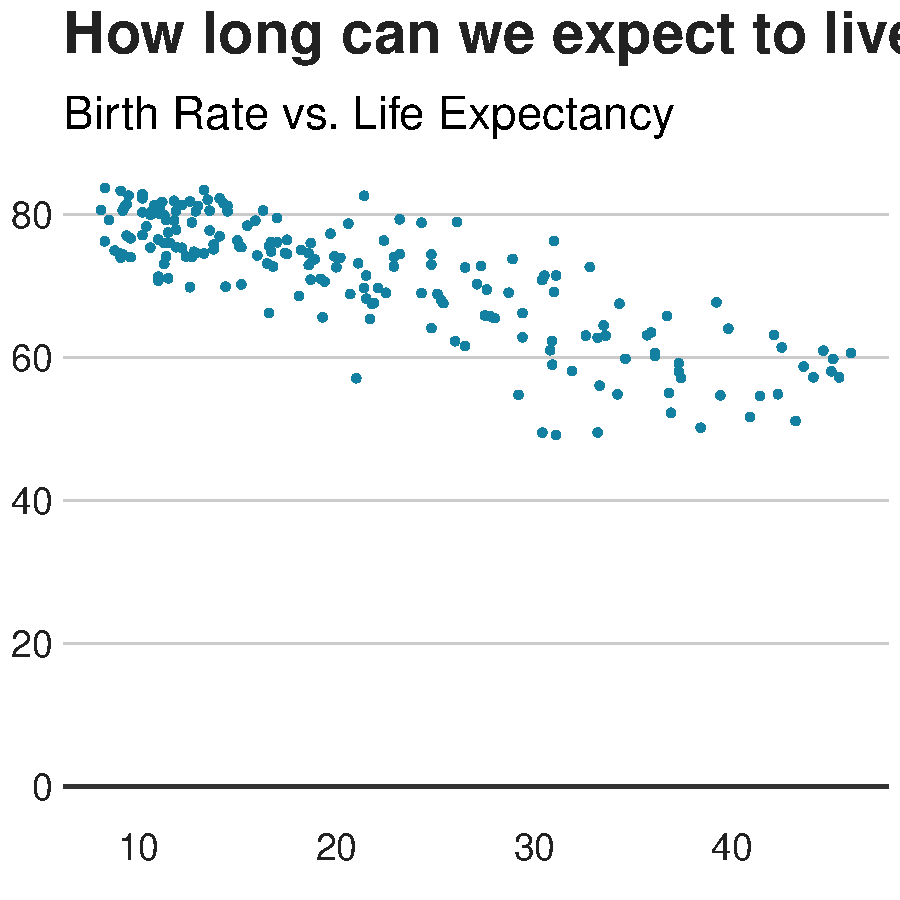
\includegraphics[width=.6\linewidth]{figure/Analysis-Rnwauto-report-4} 

}


\begin{kframe}\begin{alltt}
\hlcom{# Life vs Cancer}
\hlstd{life_exp_full} \hlopt
  \hlkwd{ggplot}\hlstd{(}\hlkwd{aes}\hlstd{(}\hlkwc{x} \hlstd{= `Cancer Rate`,}
             \hlkwc{y} \hlstd{= `Life Expectancy`))} \hlopt{+}
  \hlkwd{geom_point}\hlstd{(}\hlkwc{color} \hlstd{=} \hlstr{"#1380A1"}\hlstd{)} \hlopt{+}
  \hlkwd{geom_hline}\hlstd{(}\hlkwc{yintercept} \hlstd{=} \hlnum{0}\hlstd{,}
             \hlkwc{size} \hlstd{=} \hlnum{1}\hlstd{,}
             \hlkwc{colour} \hlstd{=} \hlstr{"#333333"}\hlstd{)} \hlopt{+}
  \hlcom{#scale_color_d3() +}
  \hlkwd{bbc_style}\hlstd{()} \hlopt{+}
  \hlkwd{labs}\hlstd{(}\hlkwc{title} \hlstd{=} \hlstr{"How long do we expect to live?"}\hlstd{,}
       \hlkwc{subtitle} \hlstd{=} \hlstr{"Cancer Rate vs. Life Expectancy"}\hlstd{)}
\end{alltt}


{\ttfamily\noindent\color{warningcolor}{\#\# Warning: Removed 70 rows containing missing values (geom\_point).}}\end{kframe}

{\centering 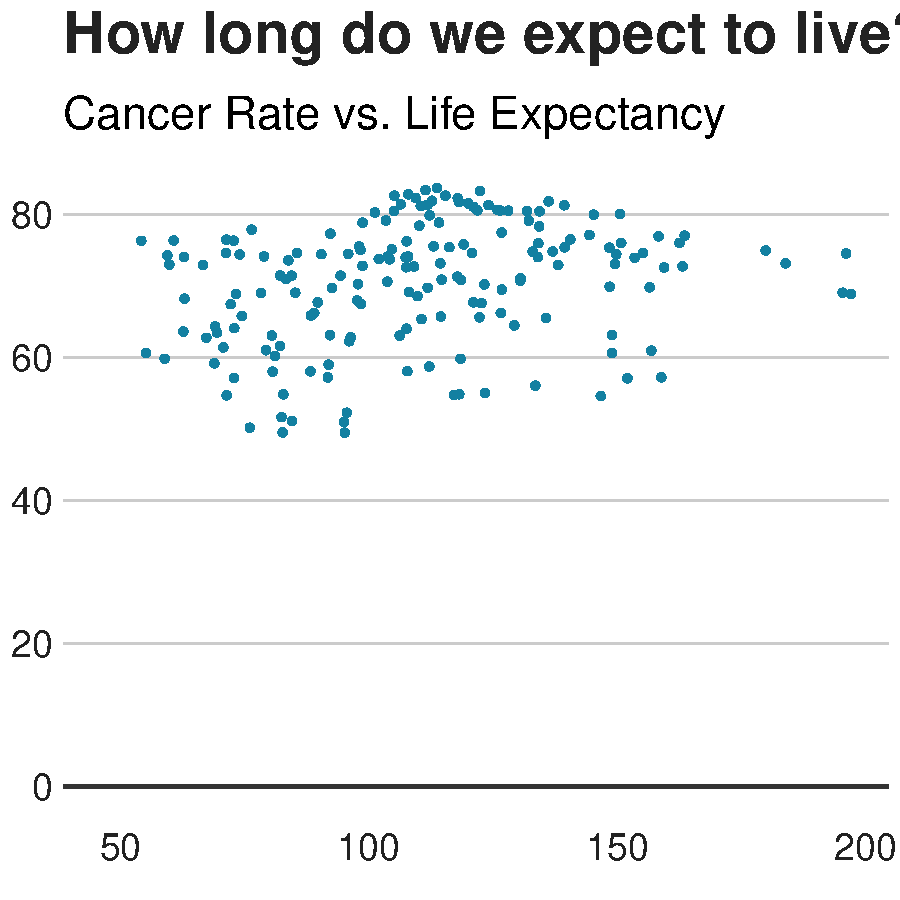
\includegraphics[width=.6\linewidth]{figure/Analysis-Rnwauto-report-5} 

}


\begin{kframe}\begin{alltt}
\hlcom{# GDP Distribution, Histogram}
\hlkwd{hist}\hlstd{(life_exp_full}\hlopt{$}\hlstd{GDP,} \hlkwc{col} \hlstd{=} \hlstr{"#1380A1"}\hlstd{)}
\end{alltt}
\end{kframe}

{\centering 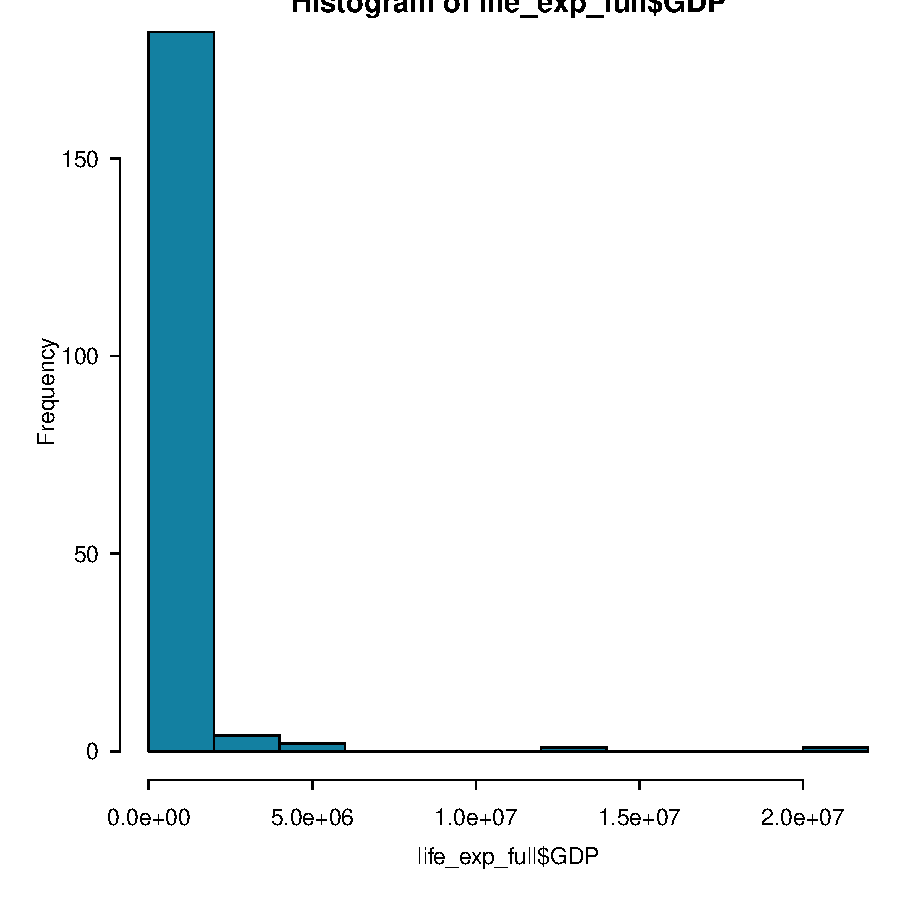
\includegraphics[width=.6\linewidth]{figure/Analysis-Rnwauto-report-6} 

}


\begin{kframe}\begin{alltt}
\hlstd{GDP_distro} \hlkwb{<-} \hlstd{life_exp_full} \hlopt
  \hlkwd{ggplot}\hlstd{(}\hlkwd{aes}\hlstd{(}\hlkwc{x} \hlstd{= GDP))} \hlopt{+}
  \hlkwd{geom_histogram}\hlstd{(}
    \hlkwc{color} \hlstd{=} \hlstr{"white"}\hlstd{,}
    \hlkwc{fill} \hlstd{=} \hlstr{"#1380A1"}\hlstd{,}
    \hlkwc{na.rm} \hlstd{=} \hlnum{TRUE}\hlstd{,}
    \hlkwc{bins} \hlstd{=} \hlnum{40}
  \hlstd{)} \hlopt{+}
  \hlkwd{geom_hline}\hlstd{(}\hlkwc{yintercept} \hlstd{=} \hlnum{0}\hlstd{,}
             \hlkwc{size} \hlstd{=} \hlnum{1}\hlstd{,}
             \hlkwc{color} \hlstd{=} \hlstr{"#333333"}\hlstd{)} \hlopt{+}
  \hlkwd{bbc_style}\hlstd{()} \hlopt{+}
  \hlkwd{scale_x_continuous}\hlstd{(}\hlkwc{labels} \hlstd{= scales}\hlopt{::}\hlstd{comma)} \hlopt{+}
  \hlkwd{labs}\hlstd{(}\hlkwc{title} \hlstd{=} \hlstr{"How GDP varies"}\hlstd{,}
       \hlkwc{subtitle} \hlstd{=} \hlstr{"Distribution of GDP (US $ Mil.)"}\hlstd{)}

\hlcom{# Save graph}
\hlkwd{finalise_plot}\hlstd{(}\hlkwc{plot_name} \hlstd{= GDP_distro,}
              \hlkwc{source} \hlstd{=} \hlstr{"Source: JNYH/Project Luther"}\hlstd{,}
              \hlkwc{save_filepath} \hlstd{=} \hlstr{"figures/GDP_distro.pdf"}\hlstd{,}
              \hlkwc{width_pixels} \hlstd{=} \hlnum{640}\hlstd{,}
              \hlkwc{height_pixels} \hlstd{=} \hlnum{450}\hlstd{)}
\end{alltt}
\end{kframe}

{\centering 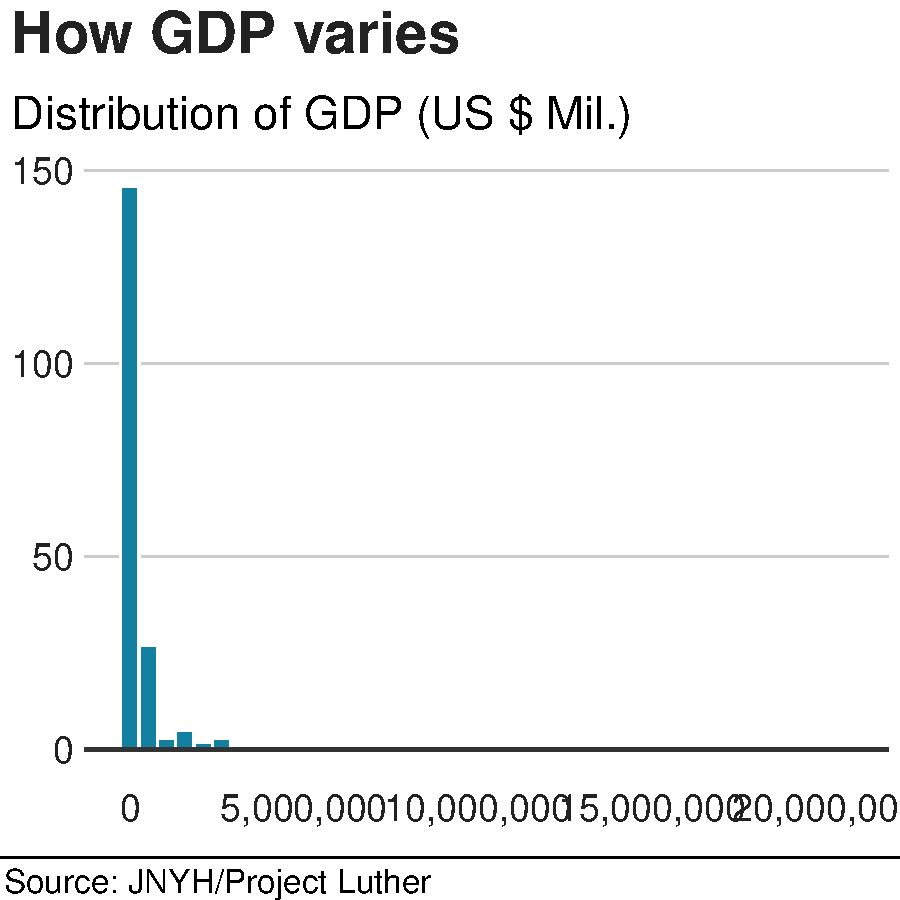
\includegraphics[width=.6\linewidth]{figure/Analysis-Rnwauto-report-7} 

}


\begin{kframe}\begin{alltt}
\hlcom{#logo_image_path = "placeholder.png")}

\hlcom{# Life vs Heart Disease}
\hlstd{life_exp_full} \hlopt
  \hlkwd{ggplot}\hlstd{(}\hlkwd{aes}\hlstd{(}\hlkwc{x} \hlstd{= `Heart Disease Rate`,}
             \hlkwc{y} \hlstd{= `Life Expectancy`))} \hlopt{+}
  \hlkwd{geom_point}\hlstd{(}\hlkwc{color} \hlstd{=} \hlstr{"#1380A1"}\hlstd{)} \hlopt{+}
  \hlkwd{geom_hline}\hlstd{(}\hlkwc{yintercept} \hlstd{=} \hlnum{0}\hlstd{,}
             \hlkwc{size} \hlstd{=} \hlnum{1}\hlstd{,}
             \hlkwc{colour} \hlstd{=} \hlstr{"#333333"}\hlstd{)} \hlopt{+}
  \hlcom{#scale_color_d3() +}
  \hlkwd{bbc_style}\hlstd{()} \hlopt{+}
  \hlkwd{labs}\hlstd{(}\hlkwc{title} \hlstd{=} \hlstr{"How long do we expect to live?"}\hlstd{,}
       \hlkwc{subtitle} \hlstd{=} \hlstr{"Heart Disease Rate vs. Life Expectancy"}\hlstd{)}
\end{alltt}


{\ttfamily\noindent\color{warningcolor}{\#\# Warning: Removed 70 rows containing missing values (geom\_point).}}\end{kframe}

{\centering 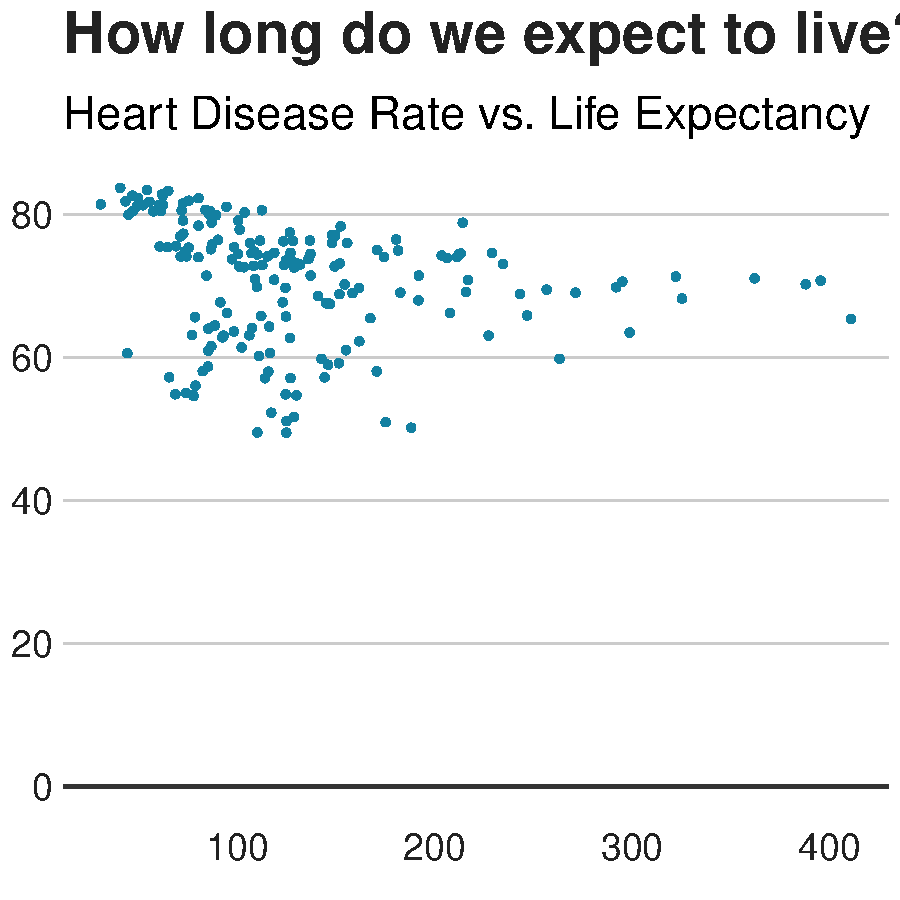
\includegraphics[width=.6\linewidth]{figure/Analysis-Rnwauto-report-8} 

}


\begin{kframe}\begin{alltt}
\hlcom{# Life vs EPI}
\hlstd{life_exp_full} \hlopt
  \hlkwd{ggplot}\hlstd{(}\hlkwd{aes}\hlstd{(}\hlkwc{x} \hlstd{= EPI,}
             \hlkwc{y} \hlstd{= `Life Expectancy`))} \hlopt{+}
  \hlkwd{geom_point}\hlstd{(}\hlkwc{color} \hlstd{=} \hlstr{"#1380A1"}\hlstd{)} \hlopt{+}
  \hlkwd{geom_hline}\hlstd{(}\hlkwc{yintercept} \hlstd{=} \hlnum{0}\hlstd{,}
             \hlkwc{size} \hlstd{=} \hlnum{1}\hlstd{,}
             \hlkwc{colour} \hlstd{=} \hlstr{"#333333"}\hlstd{)} \hlopt{+}
  \hlcom{#scale_color_d3() +}
  \hlkwd{bbc_style}\hlstd{()} \hlopt{+}
  \hlkwd{labs}\hlstd{(}\hlkwc{title} \hlstd{=} \hlstr{"How long do we expect to live?"}\hlstd{,}
       \hlkwc{subtitle} \hlstd{=} \hlstr{"EPI vs. Life Expectancy"}\hlstd{)}
\end{alltt}


{\ttfamily\noindent\color{warningcolor}{\#\# Warning: Removed 73 rows containing missing values (geom\_point).}}\end{kframe}

{\centering 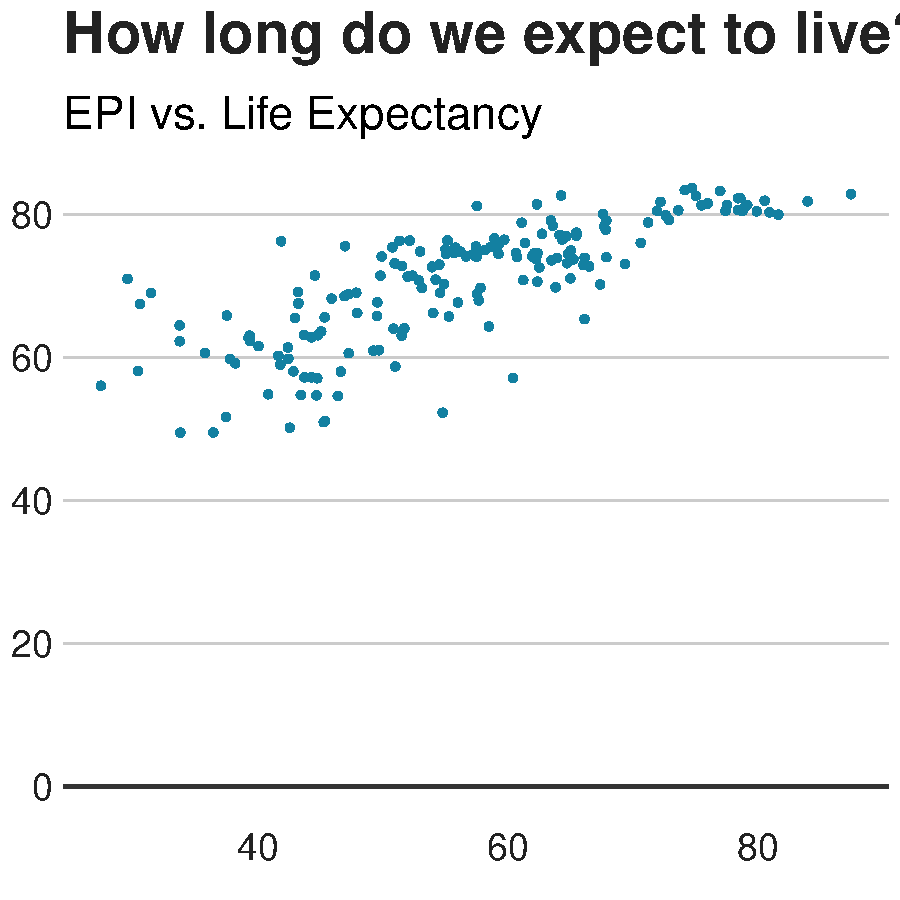
\includegraphics[width=.6\linewidth]{figure/Analysis-Rnwauto-report-9} 

}


\begin{kframe}\begin{alltt}
\hlcom{# Plot Variables v Life Expectancy ----------------------------------------}

\hlcom{# Birth}
\hlstd{life_exp_full} \hlopt
  \hlkwd{ggplot}\hlstd{()} \hlopt{+}
  \hlkwd{geom_point}\hlstd{(}
    \hlkwd{aes}\hlstd{(}\hlkwc{y} \hlstd{= `Life Expectancy`,} \hlkwc{x} \hlstd{= `Birth Rate`),}
    \hlkwc{color} \hlstd{= COLA[}\hlnum{3}\hlstd{])} \hlopt{+}
  \hlkwd{theme_clean}\hlstd{()}
\end{alltt}


{\ttfamily\noindent\color{warningcolor}{\#\# Warning: Removed 54 rows containing missing values (geom\_point).}}\end{kframe}

{\centering 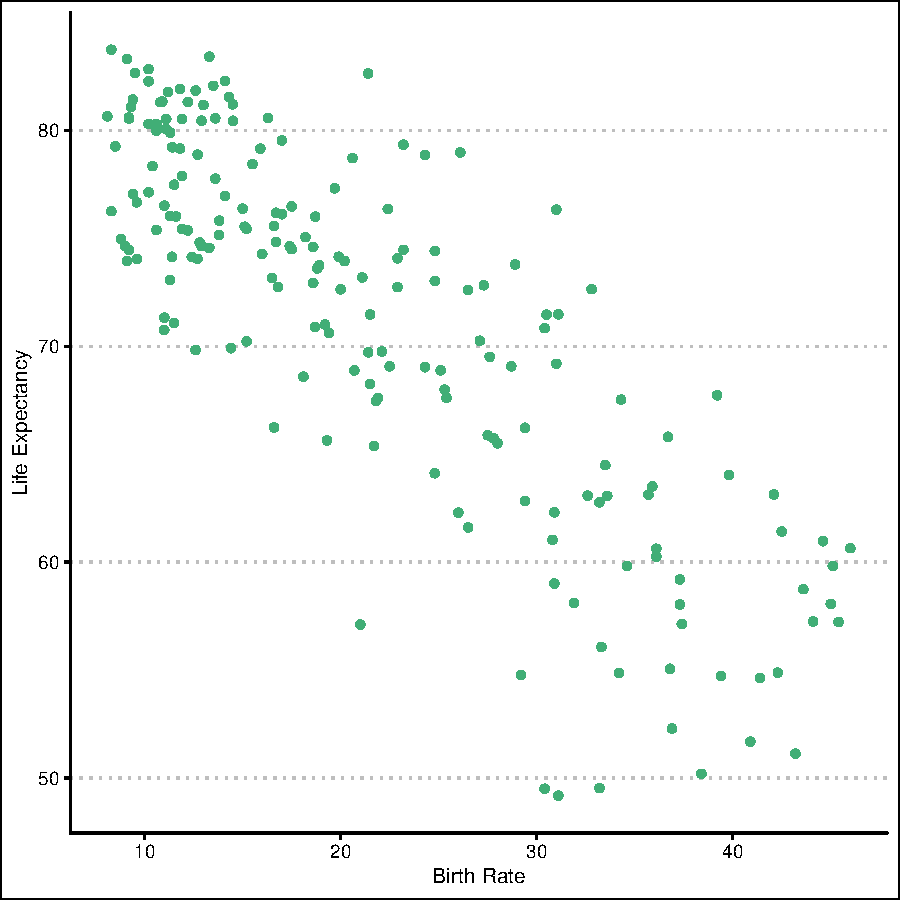
\includegraphics[width=.6\linewidth]{figure/Analysis-Rnwauto-report-10} 

}


\begin{kframe}\begin{alltt}
\hlkwd{hist}\hlstd{(life_exp_full}\hlopt{$}\hlstd{`Birth Rate`,}
     \hlkwc{xlab}   \hlstd{=} \hlstr{"Birth Rate"}\hlstd{,}
     \hlkwc{main}   \hlstd{=} \hlstr{"Histogram of Birth Rate"}\hlstd{,}
     \hlkwc{col}    \hlstd{=} \hlstr{"dodgerblue"}\hlstd{,}
     \hlkwc{border} \hlstd{=} \hlstr{"black"}\hlstd{,}
     \hlkwc{breaks} \hlstd{=} \hlnum{20}\hlstd{)}
\end{alltt}
\end{kframe}

{\centering 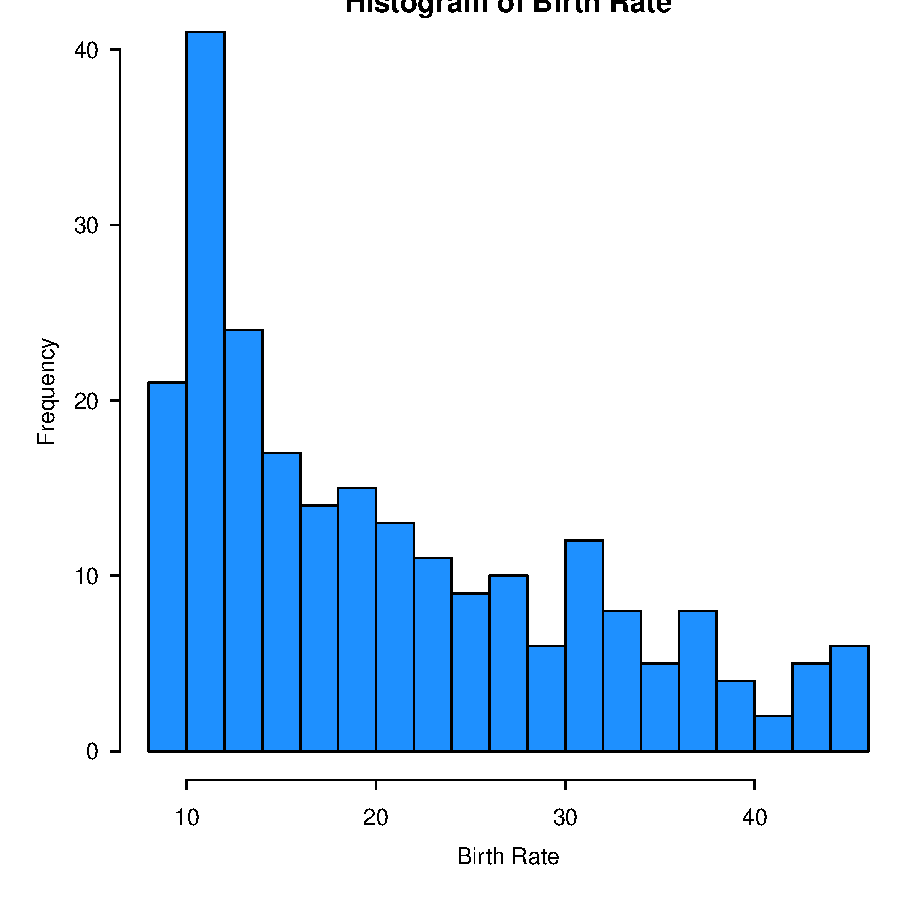
\includegraphics[width=.6\linewidth]{figure/Analysis-Rnwauto-report-11} 

}


\begin{kframe}\begin{alltt}
\hlcom{# Cancer}
\hlstd{life_exp_full} \hlopt
  \hlkwd{ggplot}\hlstd{()} \hlopt{+}
  \hlkwd{geom_point}\hlstd{(}
    \hlkwd{aes}\hlstd{(}\hlkwc{y} \hlstd{= `Life Expectancy`,} \hlkwc{x} \hlstd{= `Cancer Rate`),}
    \hlkwc{color} \hlstd{= COLA[}\hlnum{3}\hlstd{])} \hlopt{+}
  \hlkwd{theme_clean}\hlstd{()}
\end{alltt}


{\ttfamily\noindent\color{warningcolor}{\#\# Warning: Removed 70 rows containing missing values (geom\_point).}}\end{kframe}

{\centering 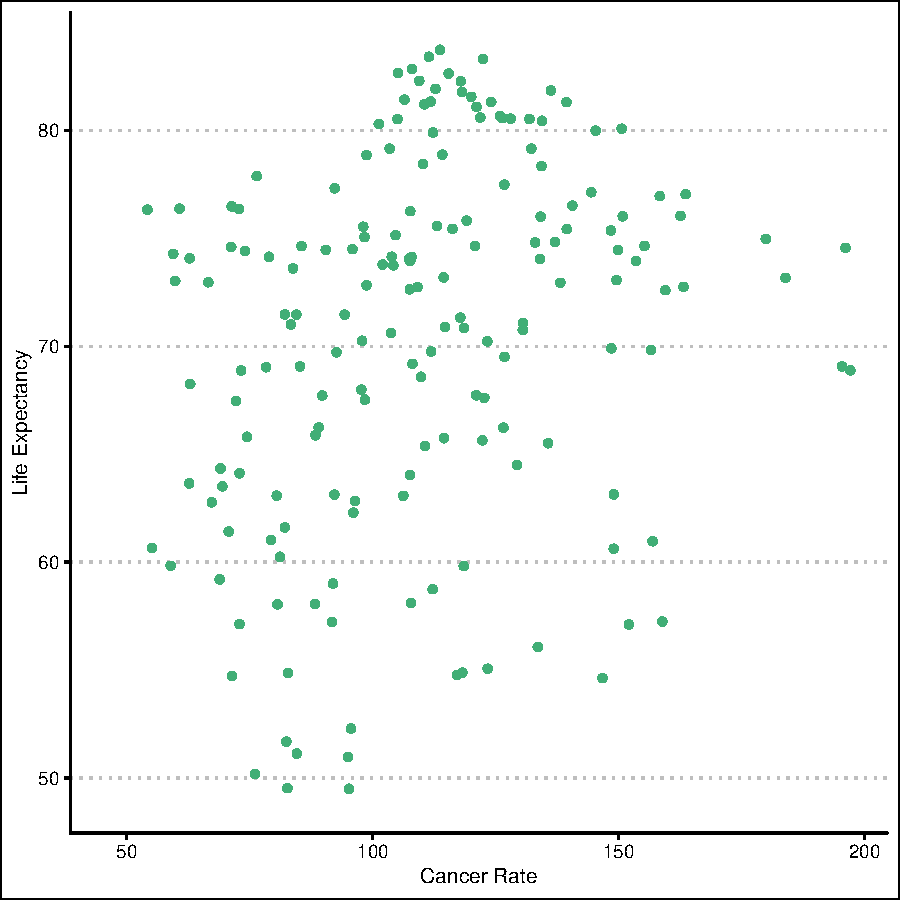
\includegraphics[width=.6\linewidth]{figure/Analysis-Rnwauto-report-12} 

}


\begin{kframe}\begin{alltt}
\hlkwd{hist}\hlstd{(life_exp_full}\hlopt{$}\hlstd{`Cancer Rate`,}
     \hlkwc{xlab}   \hlstd{=} \hlstr{"Cancer Disease"}\hlstd{,}
     \hlkwc{main}   \hlstd{=} \hlstr{"Histogram of Cancer Disease"}\hlstd{,}
     \hlkwc{col}    \hlstd{=} \hlstr{"dodgerblue"}\hlstd{,}
     \hlkwc{border} \hlstd{=} \hlstr{"black"}\hlstd{,}
     \hlkwc{breaks} \hlstd{=} \hlnum{20}\hlstd{)}
\end{alltt}
\end{kframe}

{\centering 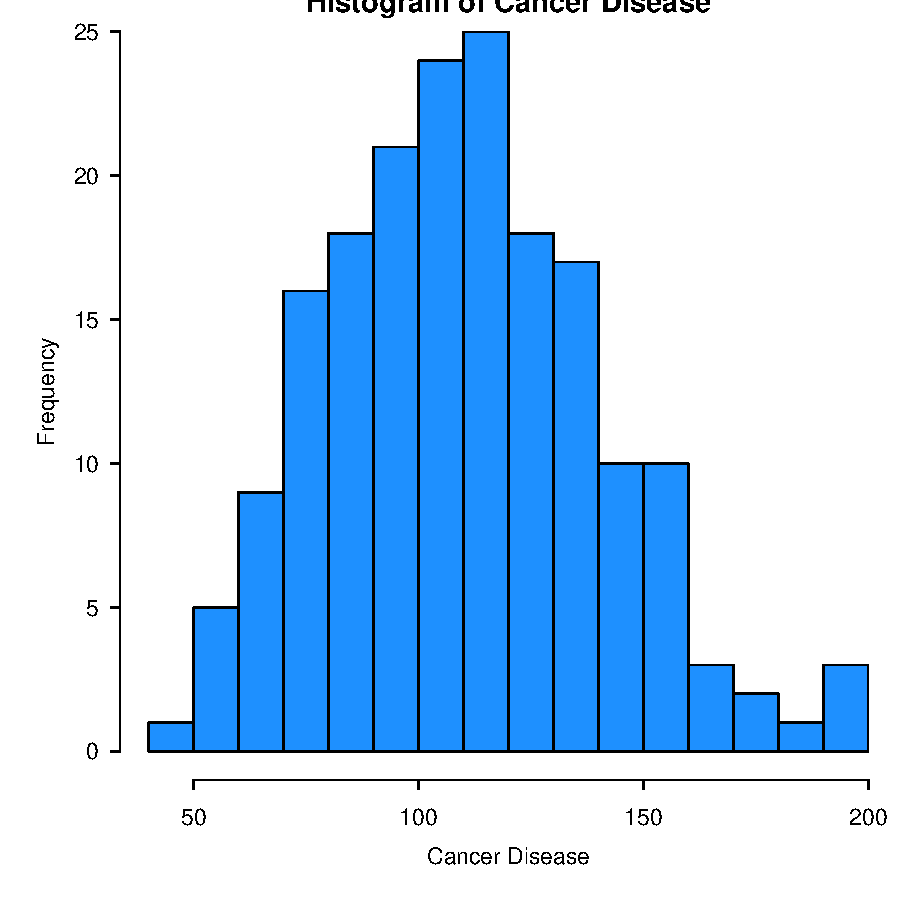
\includegraphics[width=.6\linewidth]{figure/Analysis-Rnwauto-report-13} 

}


\begin{kframe}\begin{alltt}
\hlcom{# Heart Disease}
\hlstd{life_exp_full} \hlopt
  \hlkwd{ggplot}\hlstd{()} \hlopt{+}
  \hlkwd{geom_point}\hlstd{(}
    \hlkwd{aes}\hlstd{(}\hlkwc{y} \hlstd{= `Life Expectancy`,} \hlkwc{x} \hlstd{= `Heart Disease Rate`),}
    \hlkwc{color} \hlstd{= COLA[}\hlnum{3}\hlstd{])} \hlopt{+}
  \hlkwd{theme_clean}\hlstd{()}
\end{alltt}


{\ttfamily\noindent\color{warningcolor}{\#\# Warning: Removed 70 rows containing missing values (geom\_point).}}\end{kframe}

{\centering 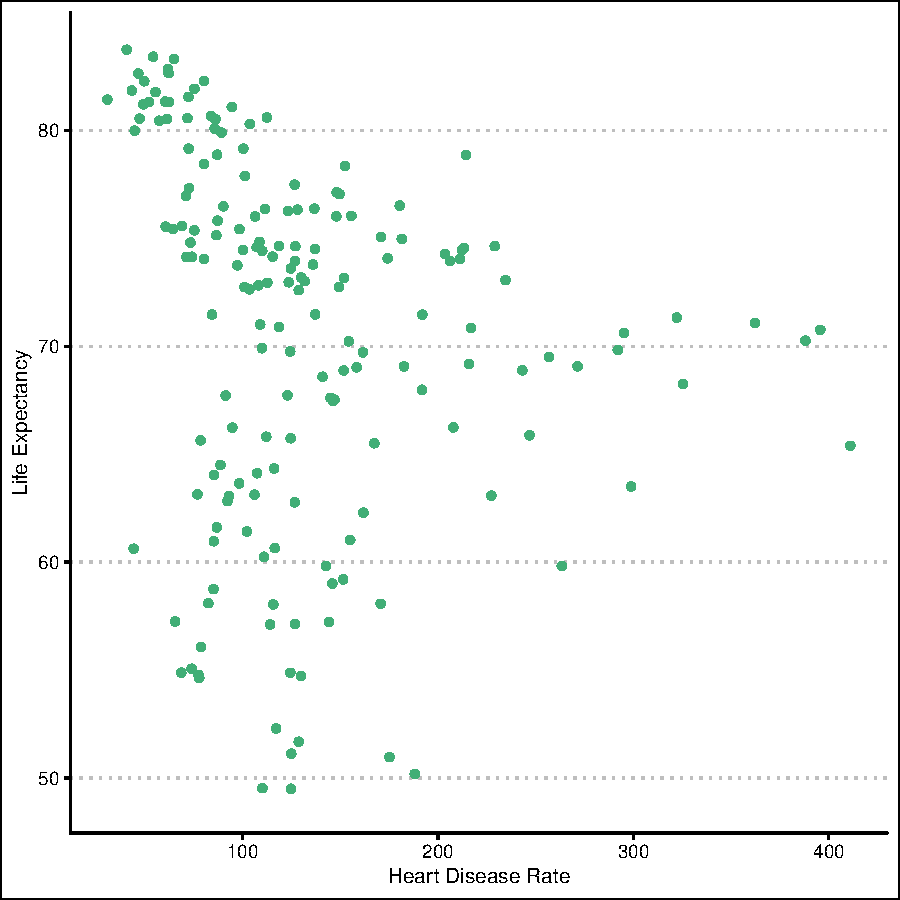
\includegraphics[width=.6\linewidth]{figure/Analysis-Rnwauto-report-14} 

}


\begin{kframe}\begin{alltt}
\hlkwd{hist}\hlstd{(life_exp_full}\hlopt{$}\hlstd{`Heart Disease Rate`,}
     \hlkwc{xlab}   \hlstd{=} \hlstr{"Heart Disease"}\hlstd{,}
     \hlkwc{main}   \hlstd{=} \hlstr{"Histogram of Heart Disease"}\hlstd{,}
     \hlkwc{col}    \hlstd{=} \hlstr{"dodgerblue"}\hlstd{,}
     \hlkwc{border} \hlstd{=} \hlstr{"black"}\hlstd{,}
     \hlkwc{breaks} \hlstd{=} \hlnum{20}\hlstd{)}
\end{alltt}
\end{kframe}

{\centering 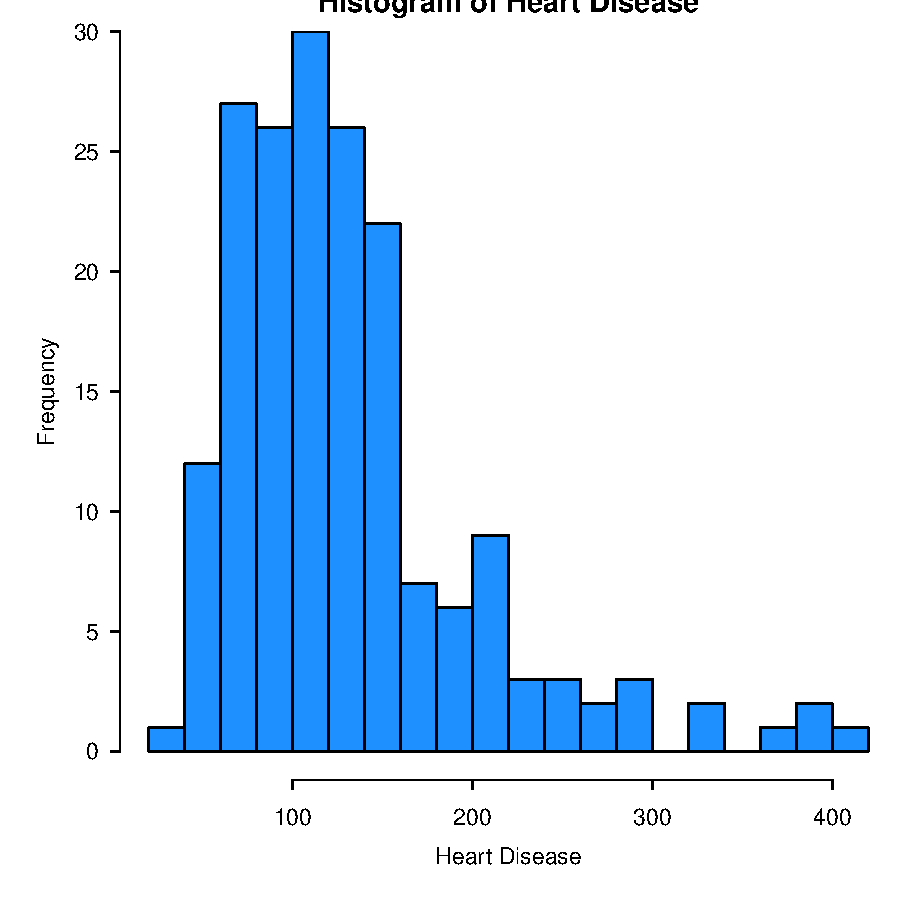
\includegraphics[width=.6\linewidth]{figure/Analysis-Rnwauto-report-15} 

}


\begin{kframe}\begin{alltt}
\hlcom{# Stroke}
\hlstd{life_exp_full} \hlopt
  \hlkwd{ggplot}\hlstd{()} \hlopt{+}
  \hlkwd{geom_point}\hlstd{(}
    \hlkwd{aes}\hlstd{(}\hlkwc{y} \hlstd{= `Life Expectancy`,} \hlkwc{x} \hlstd{= `Stroke Rate`),}
    \hlkwc{color} \hlstd{= COLA[}\hlnum{3}\hlstd{])} \hlopt{+}
  \hlkwd{theme_clean}\hlstd{()}
\end{alltt}


{\ttfamily\noindent\color{warningcolor}{\#\# Warning: Removed 70 rows containing missing values (geom\_point).}}\end{kframe}

{\centering 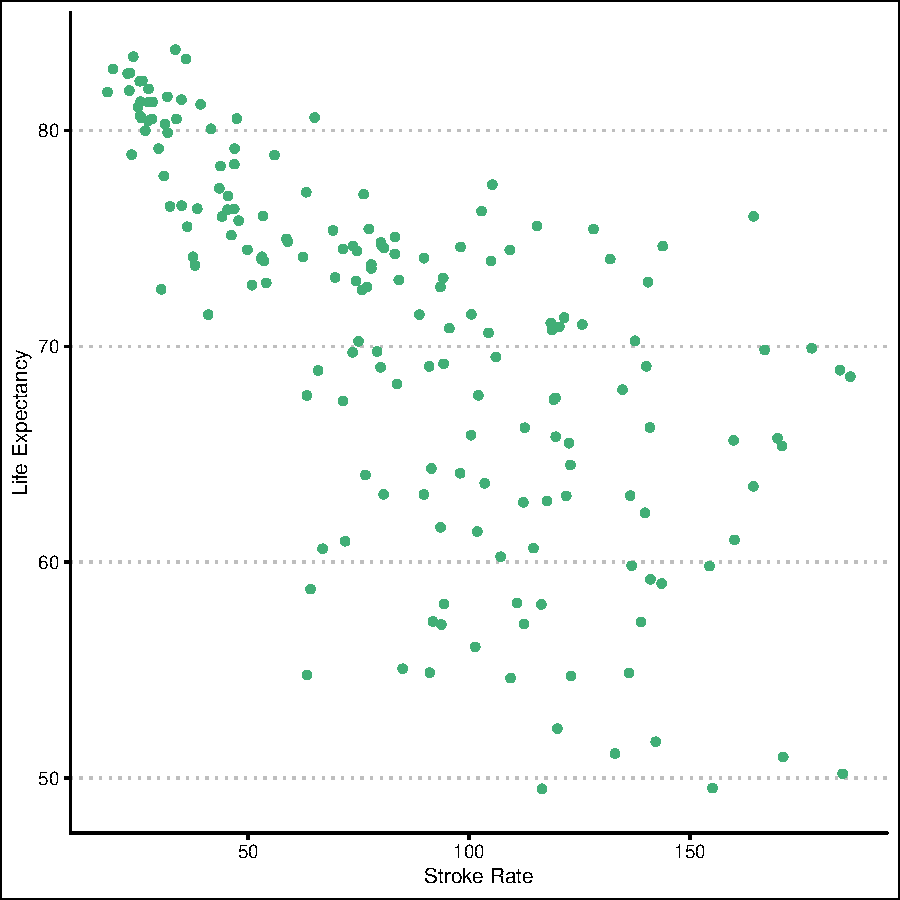
\includegraphics[width=.6\linewidth]{figure/Analysis-Rnwauto-report-16} 

}


\begin{kframe}\begin{alltt}
\hlcom{# Health Expenditure}
\hlstd{life_exp_full} \hlopt
  \hlkwd{ggplot}\hlstd{()} \hlopt{+}
  \hlkwd{geom_point}\hlstd{(}
    \hlkwd{aes}\hlstd{(}\hlkwc{y} \hlstd{= `Life Expectancy`,} \hlkwc{x} \hlstd{= `Health Expenditure`),}
    \hlkwc{color} \hlstd{= COLA[}\hlnum{3}\hlstd{])} \hlopt{+}
  \hlkwd{theme_clean}\hlstd{()}
\end{alltt}


{\ttfamily\noindent\color{warningcolor}{\#\# Warning: Removed 76 rows containing missing values (geom\_point).}}\end{kframe}

{\centering 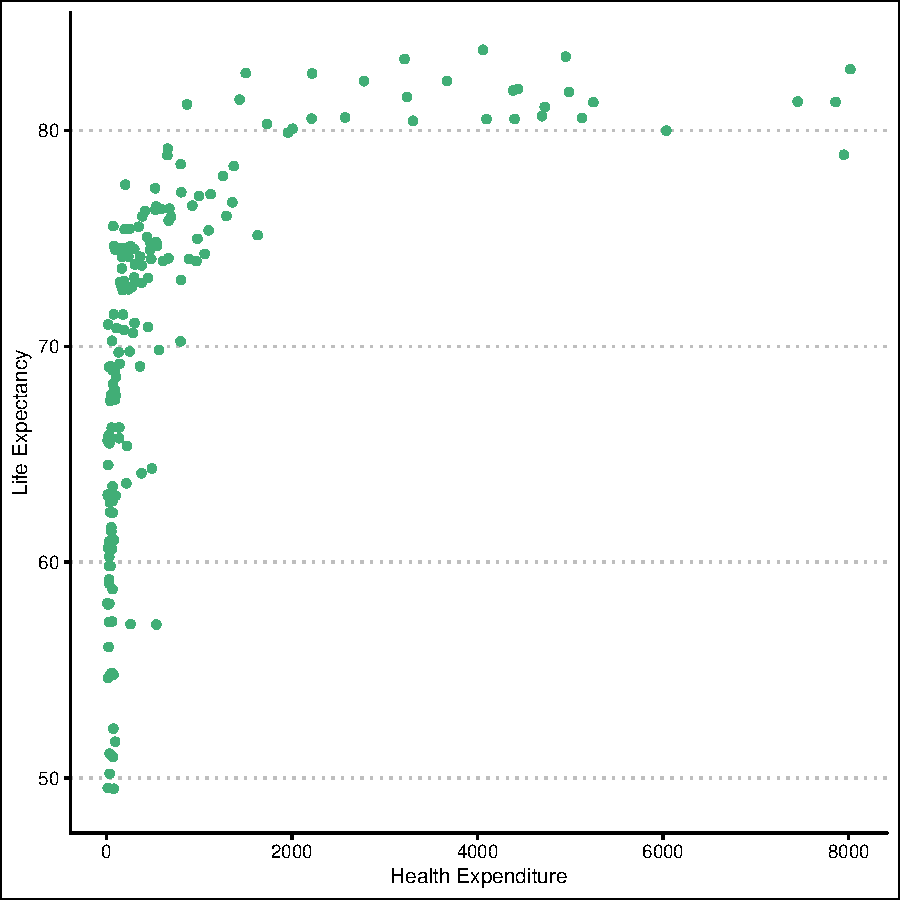
\includegraphics[width=.6\linewidth]{figure/Analysis-Rnwauto-report-17} 

}


\begin{kframe}\begin{alltt}
\hlcom{# EPI}
\hlstd{life_exp_full} \hlopt
  \hlkwd{ggplot}\hlstd{()} \hlopt{+}
  \hlkwd{geom_point}\hlstd{(}
    \hlkwd{aes}\hlstd{(}\hlkwc{y} \hlstd{= `Life Expectancy`,} \hlkwc{x} \hlstd{= EPI),}
    \hlkwc{color} \hlstd{= COLA[}\hlnum{3}\hlstd{])} \hlopt{+}
  \hlkwd{theme_clean}\hlstd{()}
\end{alltt}


{\ttfamily\noindent\color{warningcolor}{\#\# Warning: Removed 73 rows containing missing values (geom\_point).}}\end{kframe}

{\centering 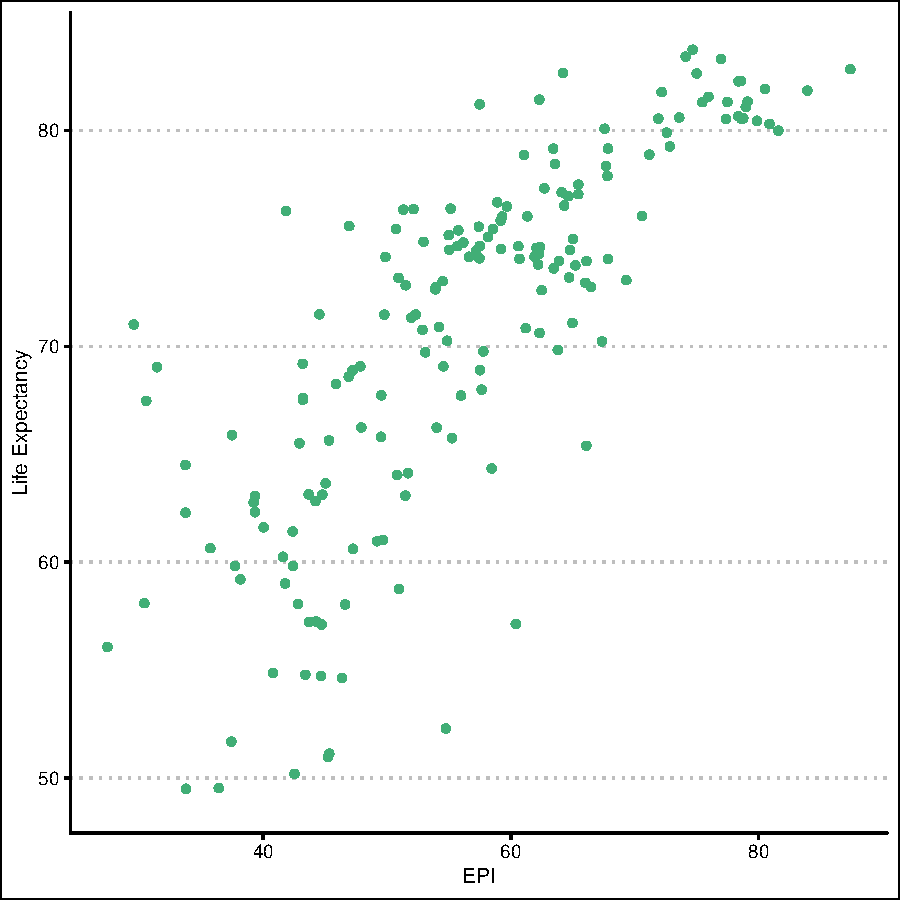
\includegraphics[width=.6\linewidth]{figure/Analysis-Rnwauto-report-18} 

}


\begin{kframe}\begin{alltt}
\hlcom{# GDP}
\hlstd{life_exp_full} \hlopt
  \hlkwd{ggplot}\hlstd{()} \hlopt{+}
  \hlkwd{geom_point}\hlstd{(}
    \hlkwd{aes}\hlstd{(}\hlkwc{y} \hlstd{= `Life Expectancy`,} \hlkwc{x} \hlstd{= GDP),}
    \hlkwc{color} \hlstd{= COLA[}\hlnum{3}\hlstd{])} \hlopt{+}
  \hlkwd{theme_clean}\hlstd{()}
\end{alltt}


{\ttfamily\noindent\color{warningcolor}{\#\# Warning: Removed 67 rows containing missing values (geom\_point).}}\end{kframe}

{\centering 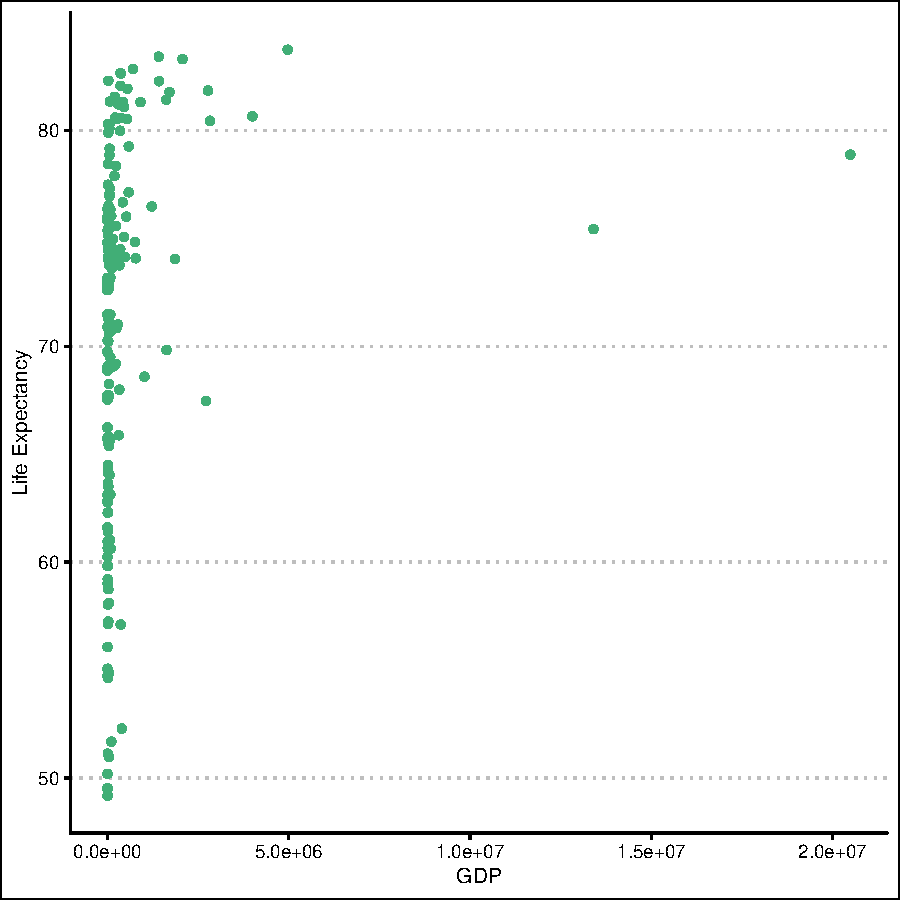
\includegraphics[width=.6\linewidth]{figure/Analysis-Rnwauto-report-19} 

}


\begin{kframe}\begin{alltt}
\hlcom{# Regressions --------------------------------------------------------------}

\hlstd{model_full} \hlkwb{<-} \hlkwd{lm}\hlstd{(}
  \hlstd{`Life Expectancy`} \hlopt{~} \hlstd{`Birth Rate`} \hlopt{+} \hlstd{`Cancer Rate`} \hlopt{+} \hlstd{`Heart Disease Rate`} \hlopt{+} \hlstd{`Stroke Rate`} \hlopt{+}  \hlstd{`Health Expenditure`} \hlopt{+} \hlstd{EPI} \hlopt{+} \hlstd{GDP,}
  \hlkwc{data} \hlstd{= life_exp_full}
\hlstd{)}

\hlcom{# Testing Model Fit -------------------------------------------------------}

\hlcom{# compare model full and model reduced.}
\hlkwd{anova}\hlstd{(model_red, model_full)}
\end{alltt}
\begin{verbatim}
## Analysis of Variance Table
## 
## Model 1: `Life Expectancy` ~ `Birth Rate` + `Stroke Rate` + `Health Expenditure` + 
##     EPI + GDP
## Model 2: `Life Expectancy` ~ `Birth Rate` + `Cancer Rate` + `Heart Disease Rate` + 
##     `Stroke Rate` + `Health Expenditure` + EPI + GDP
##   Res.Df    RSS Df Sum of Sq      F Pr(>F)
## 1    158 1995.2                           
## 2    156 1963.5  2    31.704 1.2594 0.2867
\end{verbatim}
\begin{alltt}
\hlcom{# F = 0.8399}
\hlcom{# Pr(>F) = 0.5018}
\hlcom{# Failed to reject H0: that removed var are zero.}

\hlcom{# Diagnostic Checks - Model Full -------------------------------------------}

\hlcom{# Model Summary and ANOVA}
\hlkwd{summary}\hlstd{(model_full)}
\end{alltt}
\begin{verbatim}
## 
## Call:
## lm(formula = `Life Expectancy` ~ `Birth Rate` + `Cancer Rate` + 
##     `Heart Disease Rate` + `Stroke Rate` + `Health Expenditure` + 
##     EPI + GDP, data = life_exp_full)
## 
## Residuals:
##      Min       1Q   Median       3Q      Max 
## -12.0296  -1.7375   0.0473   2.1224   7.1708 
## 
## Coefficients:
##                        Estimate Std. Error t value Pr(>|t|)    
## (Intercept)           7.637e+01  2.958e+00  25.817  < 2e-16 ***
## `Birth Rate`         -4.243e-01  3.881e-02 -10.931  < 2e-16 ***
## `Cancer Rate`        -1.507e-02  1.017e-02  -1.482    0.140    
## `Heart Disease Rate`  2.311e-03  5.156e-03   0.448    0.655    
## `Stroke Rate`        -5.894e-02  1.051e-02  -5.607 9.13e-08 ***
## `Health Expenditure` -2.225e-04  2.687e-04  -0.828    0.409    
## EPI                   1.801e-01  4.050e-02   4.448 1.64e-05 ***
## GDP                   9.325e-08  1.539e-07   0.606    0.546    
## ---
## Signif. codes:  0 '***' 0.001 '**' 0.01 '*' 0.05 '.' 0.1 ' ' 1
## 
## Residual standard error: 3.548 on 156 degrees of freedom
##   (84 observations deleted due to missingness)
## Multiple R-squared:  0.8326,	Adjusted R-squared:  0.8251 
## F-statistic: 110.8 on 7 and 156 DF,  p-value: < 2.2e-16
\end{verbatim}
\begin{alltt}
\hlkwd{anova}\hlstd{(model_full)}
\end{alltt}
\begin{verbatim}
## Analysis of Variance Table
## 
## Response: Life Expectancy
##                       Df Sum Sq Mean Sq  F value    Pr(>F)    
## `Birth Rate`           1 8213.0  8213.0 652.5242 < 2.2e-16 ***
## `Cancer Rate`          1   29.2    29.2   2.3207   0.12969    
## `Heart Disease Rate`   1  276.2   276.2  21.9426 6.072e-06 ***
## `Stroke Rate`          1  950.8   950.8  75.5445 4.620e-15 ***
## `Health Expenditure`   1   45.0    45.0   3.5773   0.06043 .  
## EPI                    1  244.8   244.8  19.4518 1.914e-05 ***
## GDP                    1    4.6     4.6   0.3669   0.54557    
## Residuals            156 1963.5    12.6                       
## ---
## Signif. codes:  0 '***' 0.001 '**' 0.01 '*' 0.05 '.' 0.1 ' ' 1
\end{verbatim}
\begin{alltt}
\hlcom{# 1 The regression function is linear (the relationship is linear).}
\hlcom{# Yes }
\hlkwd{vif}\hlstd{(model_full)}
\end{alltt}
\begin{verbatim}
##         `Birth Rate`        `Cancer Rate` `Heart Disease Rate`        `Stroke Rate` 
##             2.177726             1.214850             1.651303             2.617937 
## `Health Expenditure`                  EPI                  GDP 
##             2.712092             3.685143             1.226175
\end{verbatim}
\begin{alltt}
\hlcom{# 2 The error terms have a constant variance}

\hlcom{# Fitted vs Residuals --- model_full}
\hlkwd{plot}\hlstd{(}\hlkwd{fitted}\hlstd{(model_full),} \hlkwd{resid}\hlstd{(model_full),} \hlkwc{col} \hlstd{=} \hlstr{"grey"}\hlstd{,} \hlkwc{pch} \hlstd{=} \hlnum{20}\hlstd{,}
     \hlkwc{xlab} \hlstd{=} \hlstr{"Fitted"}\hlstd{,} \hlkwc{ylab} \hlstd{=} \hlstr{"Residuals"}\hlstd{,} \hlkwc{main} \hlstd{=} \hlstr{"Data from Full Model"}\hlstd{)}
\hlkwd{abline}\hlstd{(}\hlkwc{h} \hlstd{=} \hlnum{0}\hlstd{,} \hlkwc{col} \hlstd{=} \hlstr{"darkorange"}\hlstd{,} \hlkwc{lwd} \hlstd{=} \hlnum{2}\hlstd{)}
\end{alltt}
\end{kframe}

{\centering 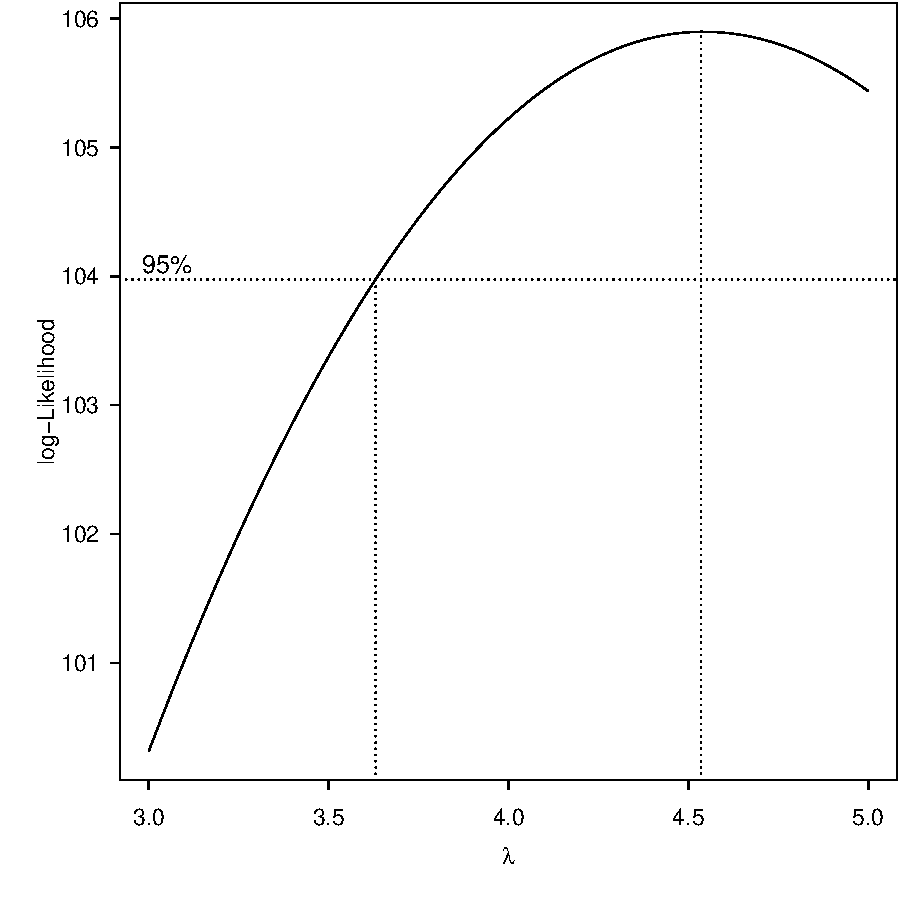
\includegraphics[width=.6\linewidth]{figure/Analysis-Rnwauto-report-20} 

}


\begin{kframe}\begin{alltt}
\hlcom{# Looks like it has a inverse parabolic shape}


\hlcom{# 3 The error terms are independent (there is no relationship among the error terms).}

\hlcom{# Breusch-Pagan Test for Homoskedasticity}
\hlkwd{bptest}\hlstd{(model_full)}
\end{alltt}
\begin{verbatim}
## 
## 	studentized Breusch-Pagan test
## 
## data:  model_full
## BP = 20.003, df = 7, p-value = 0.005563
\end{verbatim}
\begin{alltt}
\hlcom{# For model_full we see a small p-value, so we reject the null hypothesis of }
\hlcom{#     homoskedasticity is rejected and heteroskedasticity assumed.}
\hlcom{# The constant variance assumption is violated. }
\hlcom{# This matches our findings with a fitted versus residuals plot.}

\hlcom{# 4 The error terms are normally distributed}

\hlkwd{hist}\hlstd{(}\hlkwd{resid}\hlstd{(model_full),}
     \hlkwc{xlab}   \hlstd{=} \hlstr{"Residuals"}\hlstd{,}
     \hlkwc{main}   \hlstd{=} \hlstr{"Histogram of Residuals, Full Model"}\hlstd{,}
     \hlkwc{col}    \hlstd{=} \hlstr{"dodgerblue"}\hlstd{,}
     \hlkwc{border} \hlstd{=} \hlstr{"black"}\hlstd{,}
     \hlkwc{breaks} \hlstd{=} \hlnum{20}\hlstd{)}
\end{alltt}
\end{kframe}

{\centering 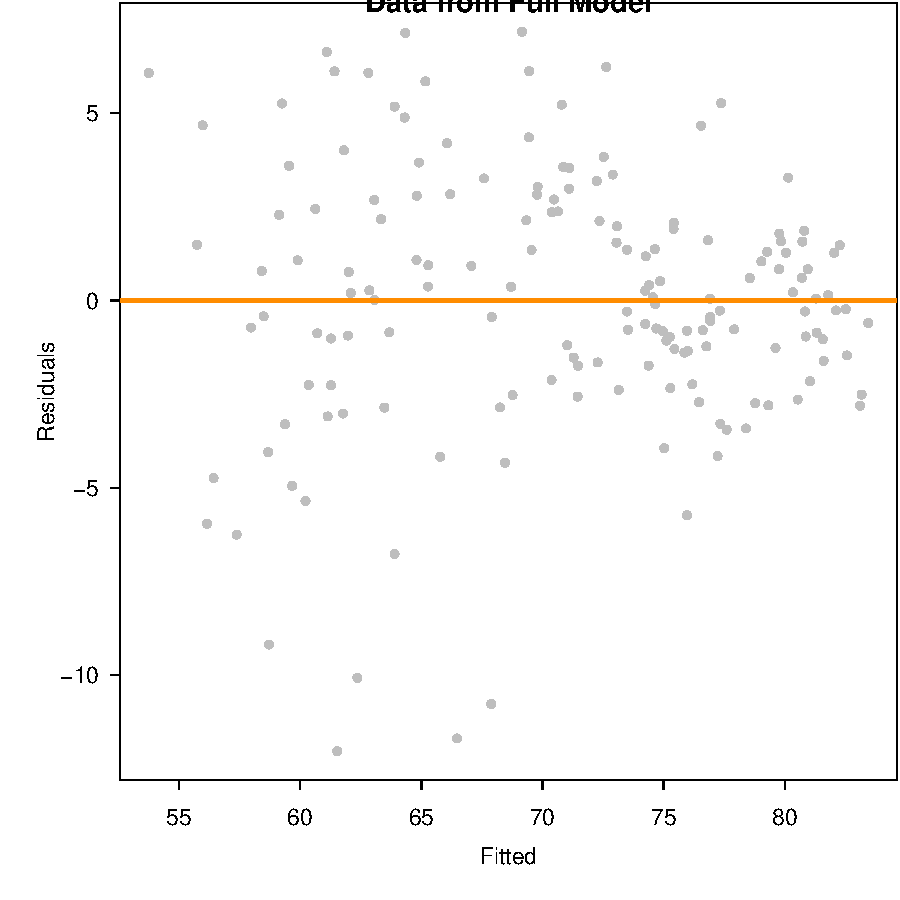
\includegraphics[width=.6\linewidth]{figure/Analysis-Rnwauto-report-21} 

}


\begin{kframe}\begin{alltt}
\hlcom{# It does have a rough bell shape, however, it also has a semi-sharp peak.}

\hlcom{# Q-Q Plot}
\hlkwd{qqnorm}\hlstd{(}\hlkwd{resid}\hlstd{(model_full),} \hlkwc{main} \hlstd{=} \hlstr{"Normal Q-Q Plot, Full Model"}\hlstd{,} \hlkwc{col} \hlstd{=} \hlstr{"darkgrey"}\hlstd{)}
\hlkwd{qqline}\hlstd{(}\hlkwd{resid}\hlstd{(model_full),} \hlkwc{col} \hlstd{=} \hlstr{"dodgerblue"}\hlstd{,} \hlkwc{lwd} \hlstd{=} \hlnum{2}\hlstd{)}
\end{alltt}
\end{kframe}

{\centering 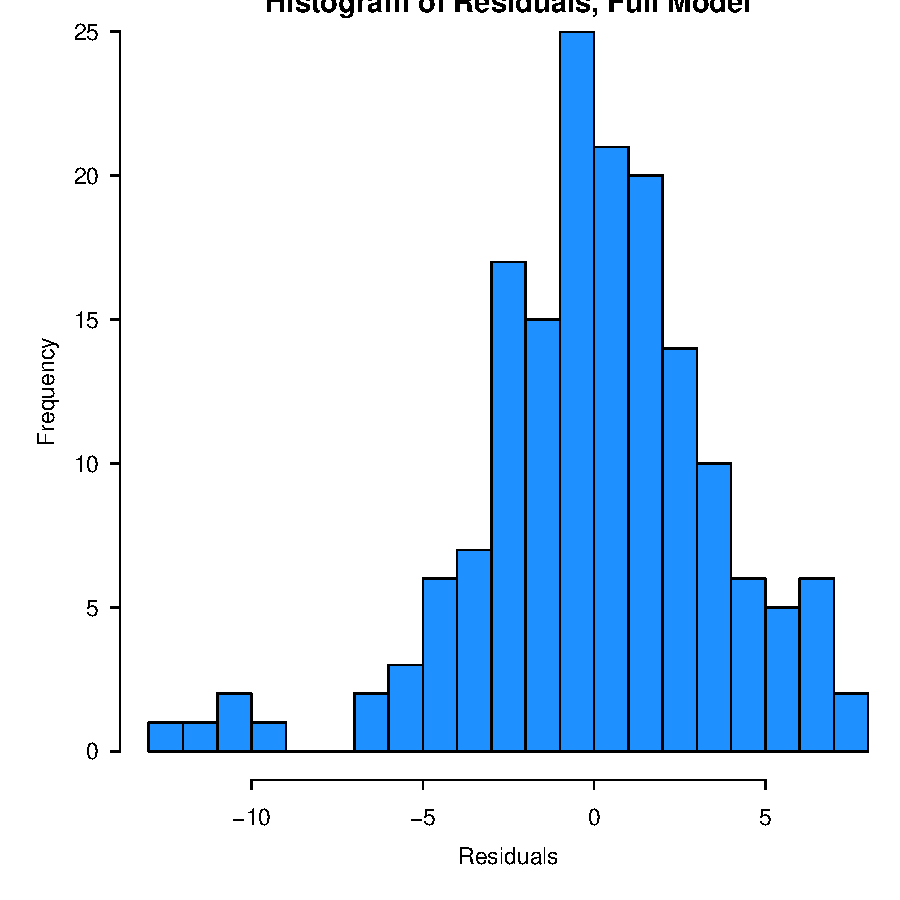
\includegraphics[width=.6\linewidth]{figure/Analysis-Rnwauto-report-22} 

}


\begin{kframe}\begin{alltt}
\hlcom{# Deviates in smaller quantiles}
\hlcom{# For Model Full, we have a suspect Q-Q plot. }
\hlcom{# We would probably not believe the errors follow a normal distribution.}

\hlcom{# Shapiro-Wilk Test}
\hlkwd{shapiro.test}\hlstd{(}\hlkwd{resid}\hlstd{(model_full))}
\end{alltt}
\begin{verbatim}
## 
## 	Shapiro-Wilk normality test
## 
## data:  resid(model_full)
## W = 0.96343, p-value = 0.0002576
\end{verbatim}
\begin{alltt}
\hlcom{# p = 7.152e-05}
\hlcom{# A small p-value indicates we believe there is only a small probability }
\hlcom{# the data could have been sampled from a normal distribution.}

\hlcom{#RK 5 Outlier Check Via Boxplots- how should we deal with those outliers? Which countries are they? }
\hlstd{outlierAssumption} \hlkwb{<-} \hlkwd{ggplot}\hlstd{(model_full,} \hlkwd{aes}\hlstd{(}\hlkwc{x}\hlstd{=}\hlkwd{fitted}\hlstd{(model_full),} \hlkwc{y}\hlstd{=}\hlkwd{resid}\hlstd{(model_full)))} \hlopt{+}
  \hlkwd{geom_boxplot}\hlstd{()} \hlopt{+}
  \hlkwd{coord_flip}\hlstd{()}
\hlstd{outlierAssumption}
\end{alltt}


{\ttfamily\noindent\color{warningcolor}{\#\# Warning: Continuous x aesthetic -- did you forget aes(group=...)?}}\end{kframe}

{\centering 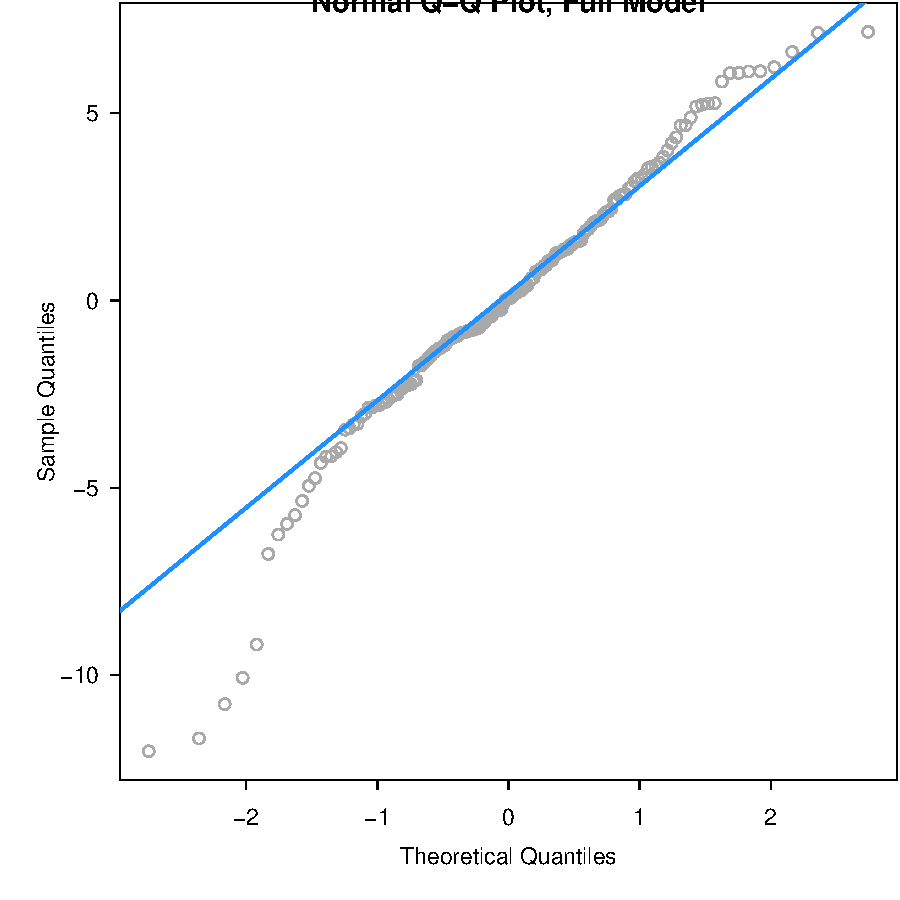
\includegraphics[width=.6\linewidth]{figure/Analysis-Rnwauto-report-23} 

}


\begin{kframe}\begin{alltt}
\hlcom{# 6 There is no important predictor that have been omitted from the model}
\hlcom{# RK I think for this one since she's just looking for a logical explanation, we can say}
\hlcom{# that there very well maybe be other factors that are contributing to the life expectancy }
\hlcom{# of a country, but it is impossible to state them all. I'm going to put a better explanation}
\hlcom{# and possible alternative predictors in the actual paper. }


\hlcom{# Diagnostic Checks - Model Reduced -------------------------------------------------------}

\hlcom{# Model Summary and ANOVA}
\hlkwd{summary}\hlstd{(model_red)}
\end{alltt}
\begin{verbatim}
## 
## Call:
## lm(formula = `Life Expectancy` ~ `Birth Rate` + `Stroke Rate` + 
##     `Health Expenditure` + EPI + GDP, data = model_full$model)
## 
## Residuals:
##      Min       1Q   Median       3Q      Max 
## -12.0656  -1.8950   0.0142   2.1378   7.9142 
## 
## Coefficients:
##                        Estimate Std. Error t value Pr(>|t|)    
## (Intercept)           7.523e+01  2.868e+00  26.228  < 2e-16 ***
## `Birth Rate`         -4.158e-01  3.763e-02 -11.052  < 2e-16 ***
## `Stroke Rate`        -5.863e-02  8.794e-03  -6.667 4.14e-10 ***
## `Health Expenditure` -2.300e-04  2.617e-04  -0.879    0.381    
## EPI                   1.725e-01  3.872e-02   4.456 1.57e-05 ***
## GDP                   8.809e-08  1.542e-07   0.571    0.569    
## ---
## Signif. codes:  0 '***' 0.001 '**' 0.01 '*' 0.05 '.' 0.1 ' ' 1
## 
## Residual standard error: 3.554 on 158 degrees of freedom
## Multiple R-squared:  0.8299,	Adjusted R-squared:  0.8245 
## F-statistic: 154.1 on 5 and 158 DF,  p-value: < 2.2e-16
\end{verbatim}
\begin{alltt}
\hlkwd{anova}\hlstd{(model_red)}
\end{alltt}
\begin{verbatim}
## Analysis of Variance Table
## 
## Response: Life Expectancy
##                       Df Sum Sq Mean Sq  F value    Pr(>F)    
## `Birth Rate`           1 8213.0  8213.0 650.3884 < 2.2e-16 ***
## `Stroke Rate`          1 1233.4  1233.4  97.6747 < 2.2e-16 ***
## `Health Expenditure`   1   34.0    34.0   2.6914    0.1029    
## EPI                    1  247.5   247.5  19.5972 1.776e-05 ***
## GDP                    1    4.1     4.1   0.3265    0.5685    
## Residuals            158 1995.2    12.6                       
## ---
## Signif. codes:  0 '***' 0.001 '**' 0.01 '*' 0.05 '.' 0.1 ' ' 1
\end{verbatim}
\begin{alltt}
\hlcom{# Fitted vs Residuals --- model_red}
\hlkwd{plot}\hlstd{(}\hlkwd{fitted}\hlstd{(model_red),} \hlkwd{resid}\hlstd{(model_red),} \hlkwc{col} \hlstd{=} \hlstr{"grey"}\hlstd{,} \hlkwc{pch} \hlstd{=} \hlnum{20}\hlstd{,}
     \hlkwc{xlab} \hlstd{=} \hlstr{"Fitted"}\hlstd{,} \hlkwc{ylab} \hlstd{=} \hlstr{"Residuals"}\hlstd{,} \hlkwc{main} \hlstd{=} \hlstr{"Data from Model Reduced"}\hlstd{)}
\hlkwd{abline}\hlstd{(}\hlkwc{h} \hlstd{=} \hlnum{0}\hlstd{,} \hlkwc{col} \hlstd{=} \hlstr{"darkorange"}\hlstd{,} \hlkwc{lwd} \hlstd{=} \hlnum{2}\hlstd{)}
\end{alltt}
\end{kframe}

{\centering 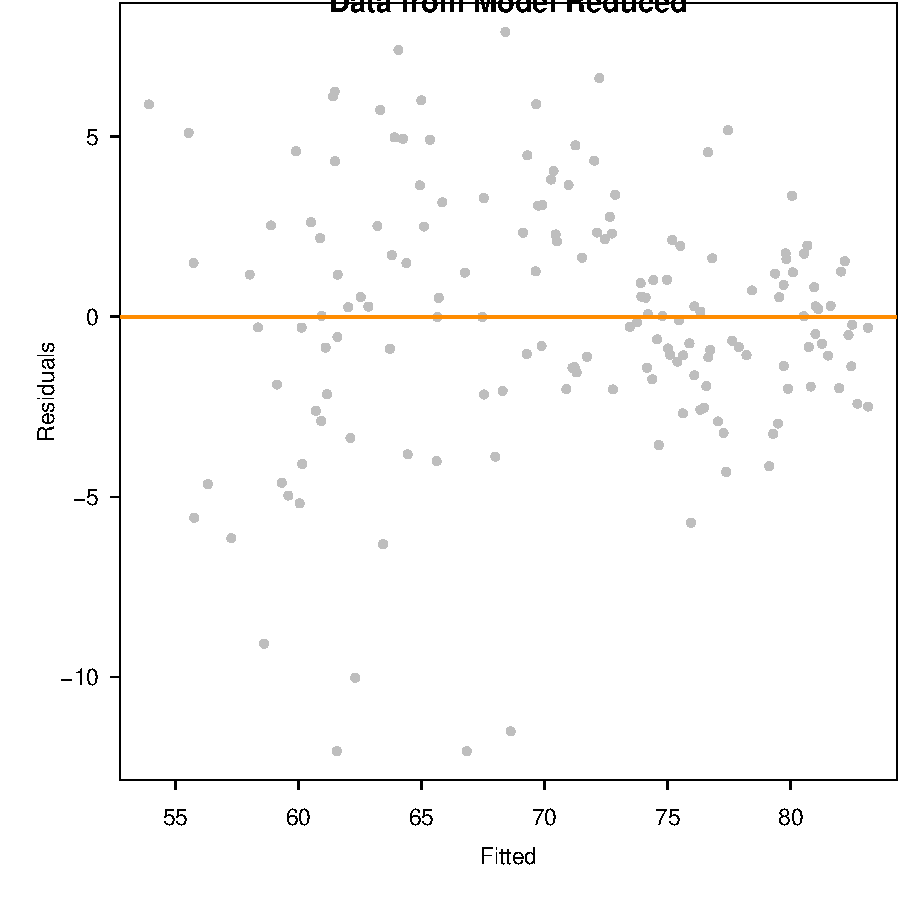
\includegraphics[width=.6\linewidth]{figure/Analysis-Rnwauto-report-24} 

}


\begin{kframe}\begin{alltt}
\hlcom{# Looks like it has a inverse parabolic shape}

\hlcom{# Breusch-Pagan Test for Homoskedasticity}
\hlkwd{bptest}\hlstd{(model_red)}
\end{alltt}
\begin{verbatim}
## 
## 	studentized Breusch-Pagan test
## 
## data:  model_red
## BP = 18.747, df = 5, p-value = 0.002142
\end{verbatim}
\begin{alltt}
\hlcom{# For model_red we see a small p-value, so we reject the null of homoskedasticity. }
\hlcom{# The constant variance assumption is violated. }
\hlcom{# This matches our findings with a fitted versus residuals plot.}

\hlcom{# Normality of errors}
\hlkwd{hist}\hlstd{(}\hlkwd{resid}\hlstd{(model_red),}
     \hlkwc{xlab}   \hlstd{=} \hlstr{"Residuals"}\hlstd{,}
     \hlkwc{main}   \hlstd{=} \hlstr{"Histogram of Residuals, Model Reduced"}\hlstd{,}
     \hlkwc{col}    \hlstd{=} \hlstr{"darkorange"}\hlstd{,}
     \hlkwc{border} \hlstd{=} \hlstr{"dodgerblue"}\hlstd{,}
     \hlkwc{breaks} \hlstd{=} \hlnum{20}\hlstd{)}
\end{alltt}
\end{kframe}

{\centering 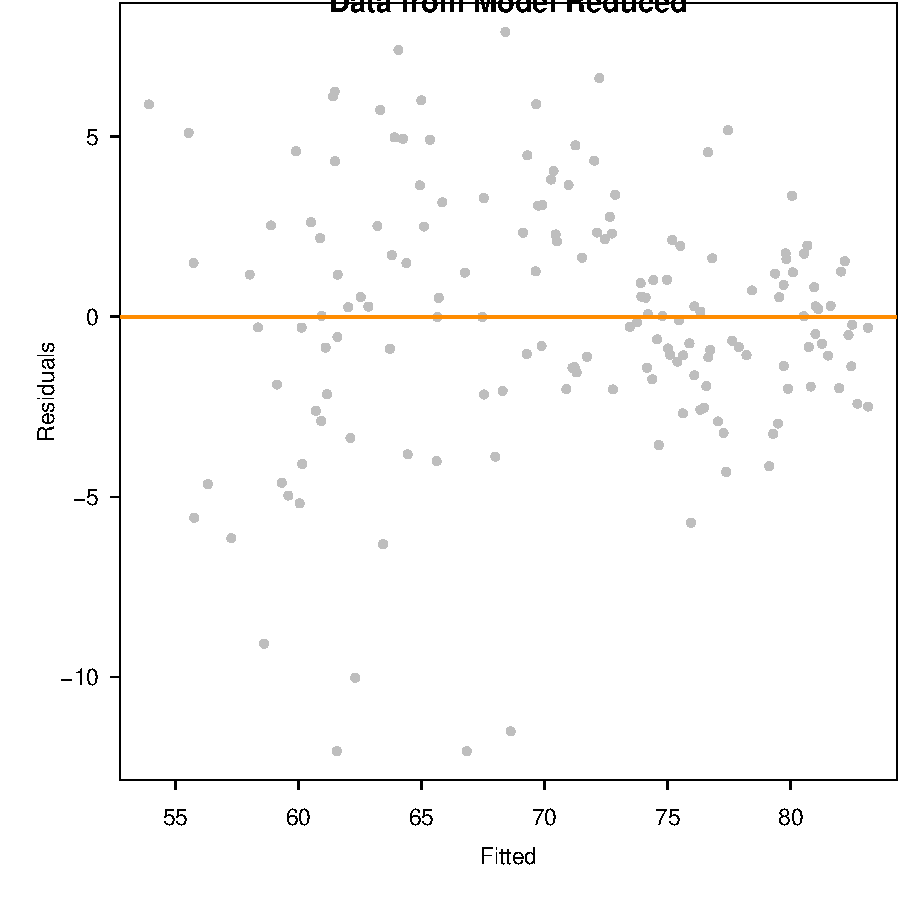
\includegraphics[width=.6\linewidth]{figure/Analysis-Rnwauto-report-25} 

}


\begin{kframe}\begin{alltt}
\hlcom{# It does have a rough bell shape, however, it also has a very sharp peak.}

\hlcom{# Q-Q Plot}
\hlkwd{qqnorm}\hlstd{(}\hlkwd{resid}\hlstd{(model_red),} \hlkwc{main} \hlstd{=} \hlstr{"Normal Q-Q Plot, Model Reduced"}\hlstd{,} \hlkwc{col} \hlstd{=} \hlstr{"darkgrey"}\hlstd{)}
\hlkwd{qqline}\hlstd{(}\hlkwd{resid}\hlstd{(model_red),} \hlkwc{col} \hlstd{=} \hlstr{"dodgerblue"}\hlstd{,} \hlkwc{lwd} \hlstd{=} \hlnum{2}\hlstd{)}
\end{alltt}
\end{kframe}

{\centering 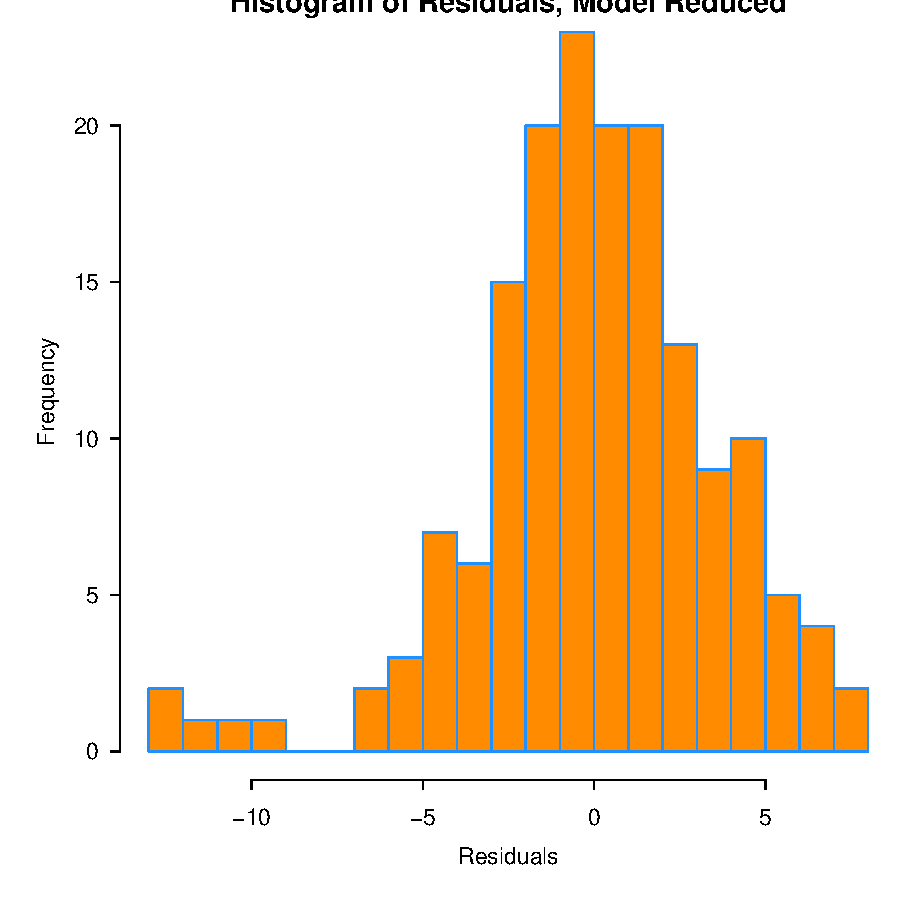
\includegraphics[width=.6\linewidth]{figure/Analysis-Rnwauto-report-26} 

}


\begin{kframe}\begin{alltt}
\hlcom{# Deviates in smaller quantiles}
\hlcom{# For Model Reduced, we have a suspect Q-Q plot. }
\hlcom{# We would probably not believe the errors follow a normal distribution.}


\hlcom{# Shapiro-Wilk Test}
\hlkwd{shapiro.test}\hlstd{(}\hlkwd{resid}\hlstd{(model_red))}
\end{alltt}
\begin{verbatim}
## 
## 	Shapiro-Wilk normality test
## 
## data:  resid(model_red)
## W = 0.96242, p-value = 0.0002042
\end{verbatim}
\begin{alltt}
\hlcom{# p = 7.152e-05}
\hlcom{# A small p-value indicates we believe there is only a small probability }
\hlcom{# the data could have been sampled from a normal distribution.}

\hlcom{# End of File -------------------------------------------------------------}
\end{alltt}
\end{kframe}
\end{knitrout}

The R session information (including the OS info, R version and all
packages used):

\begin{knitrout}
\definecolor{shadecolor}{rgb}{0.969, 0.969, 0.969}\color{fgcolor}\begin{kframe}
\begin{alltt}
\hlkwd{sessionInfo}\hlstd{()}
\end{alltt}
\begin{verbatim}
## R version 3.6.1 (2019-07-05)
## Platform: x86_64-apple-darwin15.6.0 (64-bit)
## Running under: macOS Catalina 10.15.1
## 
## Matrix products: default
## BLAS:   /System/Library/Frameworks/Accelerate.framework/Versions/A/Frameworks/vecLib.framework/Versions/A/libBLAS.dylib
## LAPACK: /Library/Frameworks/R.framework/Versions/3.6/Resources/lib/libRlapack.dylib
## 
## locale:
## [1] en_US.UTF-8/en_US.UTF-8/en_US.UTF-8/C/en_US.UTF-8/en_US.UTF-8
## 
## attached base packages:
## [1] stats     graphics  grDevices utils     datasets  methods   base     
## 
## other attached packages:
##  [1] faraway_1.0.7   MASS_7.3-51.4   scales_1.0.0    lmtest_0.9-37   zoo_1.8-6      
##  [6] bbplot_0.2      ggthemes_4.2.0  ggsci_2.9       gridExtra_2.3   forcats_0.4.0  
## [11] stringr_1.4.0   purrr_0.3.3     readr_1.3.1     tidyr_1.0.0     tibble_2.1.3   
## [16] ggplot2_3.2.1   tidyverse_1.2.1 dplyr_0.8.3     knitr_1.26     
## 
## loaded via a namespace (and not attached):
##  [1] Rcpp_1.0.3         lubridate_1.7.4    lattice_0.20-38    png_0.1-7         
##  [5] statquotes_0.2.2   assertthat_0.2.1   zeallot_0.1.0      packrat_0.5.0     
##  [9] R6_2.4.1           cellranger_1.1.0   backports_1.1.5    evaluate_0.14     
## [13] httr_1.4.0         highr_0.8          pillar_1.4.2       rlang_0.4.1       
## [17] lazyeval_0.2.2     readxl_1.3.1       minqa_1.2.4        rstudioapi_0.10   
## [21] nloptr_1.2.1       Matrix_1.2-17      labeling_0.3       splines_3.6.1     
## [25] lme4_1.1-21        tidytext_0.2.1     tinytex_0.17       munsell_0.5.0     
## [29] broom_0.5.2        compiler_3.6.1     janeaustenr_0.1.5  modelr_0.1.4      
## [33] xfun_0.11          pkgconfig_2.0.3    tidyselect_0.2.5   ggpubr_0.2.4      
## [37] crayon_1.3.4       withr_2.1.2        SnowballC_0.6.0    grid_3.6.1        
## [41] nlme_3.1-140       jsonlite_1.6       gtable_0.3.0       lifecycle_0.1.0   
## [45] magrittr_1.5       tokenizers_0.2.1   cli_1.1.0          stringi_1.4.3     
## [49] ggsignif_0.6.0     xml2_1.2.0         ellipsis_0.3.0     generics_0.0.2    
## [53] vctrs_0.2.0        cowplot_1.0.0      boot_1.3-22        wordcloud_2.6     
## [57] RColorBrewer_1.1-2 tools_3.6.1        glue_1.3.1         hms_0.5.0         
## [61] colorspace_1.4-1   rvest_0.3.4        haven_2.1.1
\end{verbatim}
\begin{alltt}
\hlkwd{Sys.time}\hlstd{()}
\end{alltt}
\begin{verbatim}
## [1] "2019-12-02 11:30:08 EST"
\end{verbatim}
\end{kframe}
\end{knitrout}


\end{document}
